% Simple thesis template for University of Stavanger
% Importing document preamble, containing all packages, document type and settings
% Setting document class and simple settings.
\documentclass[12pt,a4paper,oneside,fleqn]{article}

% geometry is for setting document margins
\usepackage[left=3.8cm,right=3.8cm,top=5cm,bottom=5cm]{geometry}

% Fonts and input encoding. Don't screw around with this, e.g. lines 5-20
\usepackage{amsmath}
\usepackage{amsfonts}
%\usepackage[adobe-utopia]{mathdesign}
\usepackage{mathdesign}
\usepackage[utf8]{inputenc}

% siunitx package is for correctly typesetting chemistry stuff. Google and check out documentation for this.
\usepackage{textcomp}
\usepackage[detect-all=true]{siunitx}
\sisetup{
        math-micro=\muup,
        math-ohm  =\Omegaup,
        text-micro={\fontfamily{mdput}\textmu},
        text-ohm  ={\fontfamily{mdput}\textohm}
}

%\renewcommand{\linespread}{1.0}

% microtype is a typesetting package that makes documents look better by doing several small adjustments
\usepackage[stretch=10]{microtype}

% booktabs is for making pretty tables
\usepackage{booktabs}			

% graphicx is for including.. graphics. The declared graphics extensions should be sufficient.					
\usepackage{graphicx}
\DeclareGraphicsExtensions{.pdf,.png,.jpg,.eps}

% setspace is used for \setstrech command used for i.e. references and table of contents. Also allows for easy setting of double line space as is customary for these kinds of documents.
\usepackage{setspace}
\setstretch{1.4}

% parskip changes the paragraph skip mechanism to a hard space between paragraphs and no indentations. This is the most "Norwegian" way to do it, so I include the command proactively... (I didn't personally use parskip in my thesis, but lots of people prefer this way of separating paragraphs)
%\usepackage{parskip}

% epstopdf converts eps pictures to pdf files which can be embedded in the document
\usepackage{epstopdf}		

% mathtools has some additional math symbols that can come in handy
\usepackage{mathtools}

% multicol and multirow are for making table cells which span several columns or rows.
\usepackage{multicol,multirow}								

% natbib handles references. Currently set up to show numbered references sorted by order of appearance.
\usepackage[sort&compress,numbers,comma]{natbib}

% xfrac is a fraction package allowing for different fractions, i.e. \sfrac and more. See documentation.
\usepackage{xfrac}	

% float package enhances float placement. See documentation!												
\usepackage{float}											

% color package is used for getting the front page lines in the correct color. No joke. Don't use colors in your documents outside of figures, people!	
\usepackage{color}
\definecolor{uisblue}{rgb}{0.471, 0.506, 0.737}

% lipsum is used for placeholder text. Add "\lipsum[1]" where you need some text and BAM!
\usepackage{lipsum}

% caption is used to get captions just right. Juuuuust right.
\usepackage[hang,justification=justified,singlelinecheck=false,labelfont=bf]{caption}		

% hyperref allows you to output digital documents with "clickables" for references, TOC etc.					
\usepackage[hidelinks]{hyperref}												

% enumitem is used for customizing list spacing
\usepackage{enumitem}					
\setlist[itemize]{itemsep=0.1mm}
\setlist[enumerate]{itemsep=0.1mm}

% mhchem is used for chemical formulas. See documentation!
\usepackage[version=3]{mhchem}		



% If you don't want any words hyphenated, activate these lines: You may get some strange results from this, like some instances of 3 short words for one line of text with oceans of space in between.

%\pretolerance 10000
%\hyphenpenalty 10000
%\exhyphenpenalty 10000


\usepackage{pdfpages}
\usepackage[english]{babel}
\usepackage{blindtext}


% Setting section title format
\usepackage[T1]{fontenc}
\usepackage{titlesec, color}

% Quotes
%\usepackage{csquotes}


\usepackage{listings}

\usepackage{graphicx}

\usepackage[toc,page]{appendix}

\usepackage{fix-cm}
\usepackage[pdftex,dvipsnames]{xcolor}
\usepackage{titlesec}

\usepackage{makecell}

\usepackage{tabu}

\usepackage{tabularx}
%\usepackage{lscape}
\usepackage{pdflscape}

% Importing custom commands for input of figures, tables, captions etc. See file for description of commands.

% This command just renews what the header of the TOC will be. I prefer "Table of Contents" over "Contents"
\renewcommand{\contentsname}{Contents}
% \renewcommand{\tablesname}{Tables}
%\renewcommand{\figuresname}{Contets}

% For referencing figures, tables and equations consistently.
\newcommand{\figref}[1]{Figure~\ref{#1}}	% Referencing a figure
\newcommand{\tabref}[1]{Table~\ref{#1}}		% Referencing a table
\newcommand{\eref}[1]{Equation~\ref{#1}}	% Referencing an equation
\newcommand{\secref}[1]{Section~\ref{#1}}	% Referencing a section

% Command for inserting figure with caption. Requires 5 arguments:
%
%	1) Location/Name of picture file
%	2) Width of picture in document as a fraction of textwidth
%	3) Label of figure (for referencing)
%	4) Figure caption
%	5) Float placement
\newcommand{\fig}[5]{
	\begin{figure}[#5]										% Figure placement
		\includegraphics[width=#2\textwidth]{figures/#1}	% Figure size and name
		\caption{#4}										% Figure caption	 (short, long)
		\label{#3}											% Reference label
	\end{figure}
}

% Command for inserting figure without caption (used in front page) and has 3 arguments:
%
%	1) Name of picture file
%	2) Width of picture in document as a fraction of textwidth
%	3) Label
\newcommand{\fignc}[3]{
	\begin{figure}[H]										% Figure placement
		\includegraphics[width=#2\textwidth]{figures/#1}	% Figure size and name
		\label{#3}											% Figure label
	\end{figure}
}

% Command for inserting table with caption. Requires 5 arguments:
%
%	1) Number of and type of columns (i.e. ccc for 3 basic centered columns)
%	2) Label of table (for referencing)
%	3) Table caption
%	4) Float placement
%	5) Table data
\newcommand{\tab}[5]{
 \vspace{3mm}							% Bit of spacing before the table
	\begin{table}[#4]					% Table placement

		\caption{#3}						% Table caption (short, long)
	\begin{tabular}{#1}					% Table properties, structure
	#5									% Table data
	\end{tabular}		
	\label{#2}							% Reference label
	\end{table}
}

\newcommand{\comment}[1]{}


\usepackage{floatpag,mwe}


%\renewcommand{\sfdefault}{qag}
\usepackage{packages/kbordermatrix}

\usepackage{url}
%\usepackage{hyperref}
%\usepackage[hidelinks]{hyperref}

\usepackage[justification=centering]{caption}
\usepackage{beramono}

\usepackage{listings}

%\geometry{left=1.0in,right=1.0in,top=1.0in,bottom=1.0in }

\comment{
\newenvironment{Description}{\list{}{%
    \let\makelabel\descriptionlabel    % this comes from the original description environment
    \setlength{\rightmargin-1cm}{}% this comes from the original quote environment
    \setlength{\labelwidth}{0pt}%          this is new
    }}{\endlist}
    }
    
\newlist{Description}{description}{1}
\setlist[Description]{labelindent=0.8\parindent,leftmargin=0.8\parindent}

\definecolor{light_gray}{gray}{0.95}
\definecolor{mypink2}{RGB}{137, 31, 127}

\usepackage{courier}
\usepackage[font=footnotesize,labelfont=bf]{caption}


\lstset{
  language=Python,
  %belowcaptionskip=4mm,
  belowskip=4mm,
  showstringspaces=false,
  columns=flexible,
  backgroundcolor=\color{light_gray},
  basicstyle={\scriptsize\ttfamily},
  numberstyle=\scriptsize\color{black},
  keywordstyle=\bfseries,
  stringstyle=\bfseries,
  commentstyle=\textit,
  breaklines=true,
  numbers=left,
  breakatwhitespace=true,
  tabsize=3,
  captionpos=b,
  frame=tb,
  framextopmargin=1pt,
  framexbottommargin=1pt,
  framexleftmargin=1pt,
  framexrightmargin=1pt,
  %framexleftmargin=18.4pt,
  xleftmargin=3.4ex
}

%\DeclareCaptionFormat{listing}{\rule{\dimexpr\textwidth\relax}{1.4pt}\par\vskip1pt#1#2#3}
\DeclareCaptionFormat{listing}{{\scriptsize}{#1#2#3}}
\captionsetup[lstlisting]{format=listing}


\renewcommand\lstlistingname{Listing}
\renewcommand\lstlistlistingname{Listings}

\newcommand\toolname{OptiRun}

\DeclareMathAlphabet{\cmsy}{OMS}{cmsy}{m}{n}

\newcommand{\PRLsep}{\noindent\makebox[\linewidth]{\resizebox{0.3333\linewidth}{1pt}{$\bullet$}}\bigskip}

\newcommand\fakesc[1]{\uppercase{{\scriptsize #1}}}


\usepackage{xstring} % needed for IfEqCase
\usepackage{forloop}

\newcounter{sccounter}
\newcounter{tempStringLength}

\newcommand{\betterfakesc}[1]{%
    % this \betterfakesc command requires these two packages:
    %   xstring
    %   forloop
    %
    % First, we obtain the length of the input string.
    \StrLen{#1}[\stringLength]%
    %
    % Our main forloop will be using a condition of “while less than \stringLength”,
    % so we’ll need to increase \stringLength by 1 so the forloop will be able to iterate 
    % over the entire string. we’ll use a temporary counter tempStringLength to make
    % this increase. That’s what the next three lines are about.
    \setcounter{tempStringLength}{\stringLength}%
    \addtocounter{tempStringLength}{1}%
    \def\stringLength{\arabic{tempStringLength}}%
    %
    % Here is our main loop. We iterate over the characters in the input string,
    % and the currentLetter is compared to the case rules we have defined. Basically
    % if the currentLetter is any of the lowercase a-z letters, then we apply a 
    % “fake small caps” effect to it and output it.
    \forloop[1]{sccounter}{1}{\value{sccounter}<\stringLength}{%
        \StrChar{#1}{\value{sccounter}}[\currentLetter]%
        %
        \IfEqCase*{\currentLetter}{%
        % The lines below are the rules. Obviously more could be added.
        {a}{{\uppercase{\scriptsize a}}}%
        {b}{{\uppercase{\scriptsize b}}}%
        {c}{{\uppercase{\scriptsize c}}}%
        {d}{{\uppercase{\scriptsize d}}}%
        {e}{{\uppercase{\scriptsize e}}}%
        {f}{{\uppercase{\scriptsize f}}}%
        {g}{{\uppercase{\scriptsize g}}}%
        {h}{{\uppercase{\scriptsize h}}}%
        {i}{{\uppercase{\scriptsize i}}}%
        {j}{{\uppercase{\scriptsize j}}}%
        {k}{{\uppercase{\scriptsize k}}}%
        {l}{{\uppercase{\scriptsize l}}}%
        {m}{{\uppercase{\scriptsize m}}}%
        {n}{{\uppercase{\scriptsize n}}}%
        {o}{{\uppercase{\scriptsize o}}}%
        {p}{{\uppercase{\scriptsize p}}}%
        {q}{{\uppercase{\scriptsize q}}}%
        {r}{{\uppercase{\scriptsize r}}}%
        {s}{{\uppercase{\scriptsize s}}}%
        {t}{{\uppercase{\scriptsize t}}}%
        {u}{{\uppercase{\scriptsize u}}}%
        {v}{{\uppercase{\scriptsize v}}}%
        {w}{{\uppercase{\scriptsize w}}}%
        {x}{{\uppercase{\scriptsize x}}}%
        {y}{{\uppercase{\scriptsize y}}}%
        {z}{{\uppercase{\scriptsize z}}}%
        }%
        % if our \currentLetter isn’t any of the letters we have rules for,
        % then just output it now
        [{\currentLetter}]%
    }%
}

%%%

\usepackage{fancyhdr}

\pagestyle{fancy}
\renewcommand{\sectionmark}[1]{\markright{\thesection\ #1}}

\fancyhf{}

\rhead{\fancyplain{}{}} % predefined ()
\lhead{\fancyplain{}{\slshape \nouppercase \rightmark}} % 1. sectionname, 1.1 subsection name etc
%\lhead{\fancyplain{}{\betterfakesc \rightmark}} % 1. sectionname, 1.1 subsection name etc
\cfoot{\fancyplain{}{\thepage}}

\comment{
    \fancypagestyle{plain}{%
        \fancyhf{}% Clear header/footer
        \fancyfoot[OR]{\thepage}%
        \fancyfoot[EL]{\thepage}%
        \renewcommand{\headrulewidth}{0pt}%
    }
}

% Option to only compile parts of the document. Shortens compiling time and makes longer documents more manageable
% Remove comment from the parts you want to compile, as well as opening/closing of command
% Comment out entire command for compiling full document

%\includeonly{
%chapters/abstract,						
%chapters/acknowledgement,
%chapters/introduction,
%chapters/template,
%chapters/example
%}



%\newcommand{\hsp}{\hspace{20pt}}
%\titleformat{\section}[hang]{\Huge\bfseries}{\thesection\hsp\textcolor{black}}{0pt}{\Huge\bfseries}



\definecolor{gray75}{gray}{0.55}
\newcommand{\hsp}{\hspace{0pt}}
\titleformat{\section}[hang]
    {\vspace*{2.4cm}\flushright\fontseries{b}\fontsize{60}{0}\selectfont}
    {\fontseries{b}\fontsize{115}{40}\selectfont\textcolor{gray75}\thesection\hsp}
    {0em}
    {\\\fontsize{25}{100}\emph}[]

\titlespacing*{\section}{0cm}{0cm}{1.7cm}

\renewcommand{\baselinestretch}{1} 

%%%%%%%%%%%%%%%%%%%%%%%%%%%%%%%%%%%%%%%%%%%%%%%%%%%

\usepackage{xargs}                      % Use more than one optional parameter in a new commands
%\usepackage[pdftex,dvipsnames]{xcolor}  % Coloured text etc.
% 
\usepackage[colorinlistoftodos,prependcaption,textsize=tiny]{todonotes}
\newcommandx{\unsure}[2][1=]{\todo[linecolor=red,backgroundcolor=red!25,bordercolor=red,#1]{#2}}
\newcommandx{\change}[2][1=]{\todo[linecolor=blue,backgroundcolor=blue!25,bordercolor=blue,#1]{#2}}
\newcommandx{\info}[2][1=]{\todo[linecolor=OliveGreen,backgroundcolor=OliveGreen!25,bordercolor=OliveGreen,#1]{#2}}
\newcommandx{\improvement}[2][1=]{\todo[linecolor=Plum,backgroundcolor=Plum!25,bordercolor=Plum,#1]{#2}}
\newcommandx{\thiswillnotshow}[2][1=]{\todo[disable,#1]{#2}}


%\renewcommand{\sectionheadstartvskip}{\vspace*{-2\baselineskip}}

%\usepackage[a4paper, total={6in, 8in}]{geometry}

\usepackage[T1]{fontenc}


%\renewcommand{\UrlFont}{\scriptsize \ttfamily}
\renewcommand{\UrlFont}{\ttfamily}

% ********** DOCUMENT BEGINS **********
\begin{document}		%The document is defined within this environment

%\thispagestyle{empty}

\begin{Huge}TODO notes\end{Huge}

\vspace{0.6cm}

\todo[inline]{TODO inline}
\unsure[inline]{UNSURE inline}
\improvement[inline]{IMPROVEMENT inline}
\info[inline]{INFO inline}
\change[inline]{CHANGE inline}

\vspace{0.6cm}

\todo[inline] {
    TODO when finished:\\
    - Search for: [, [? ], ??, [...], [source]\\
    - Remove all todo notes\\
    - Check headers and footers (Special pages: empty, first pages of chapters, contents, etc: plain, otherwise standard)\\
    - Add official UiS front page\\
    - Add custom front page\\
    - Check that EVERYTHING is included (abstract, acknowledgements, toc, other lists, all chapters, bibliography, appendix)\\
    - Check bibliography format - Double check all sources? Include page numbers?\\
    - Check that enough sources are included, and that there aren't any information that should have a source, but doesn't.\\
    - Change [tool name] command to actual tool name (and oh, come up with a great tool name too, please)\\
    - Check that there is no space between tool name and special characters, and that there \emph{is} space between tool name and next word. (use \ space command) \\
    - SPELL-CHECK!!!
}


    
    % Include UiS front page
    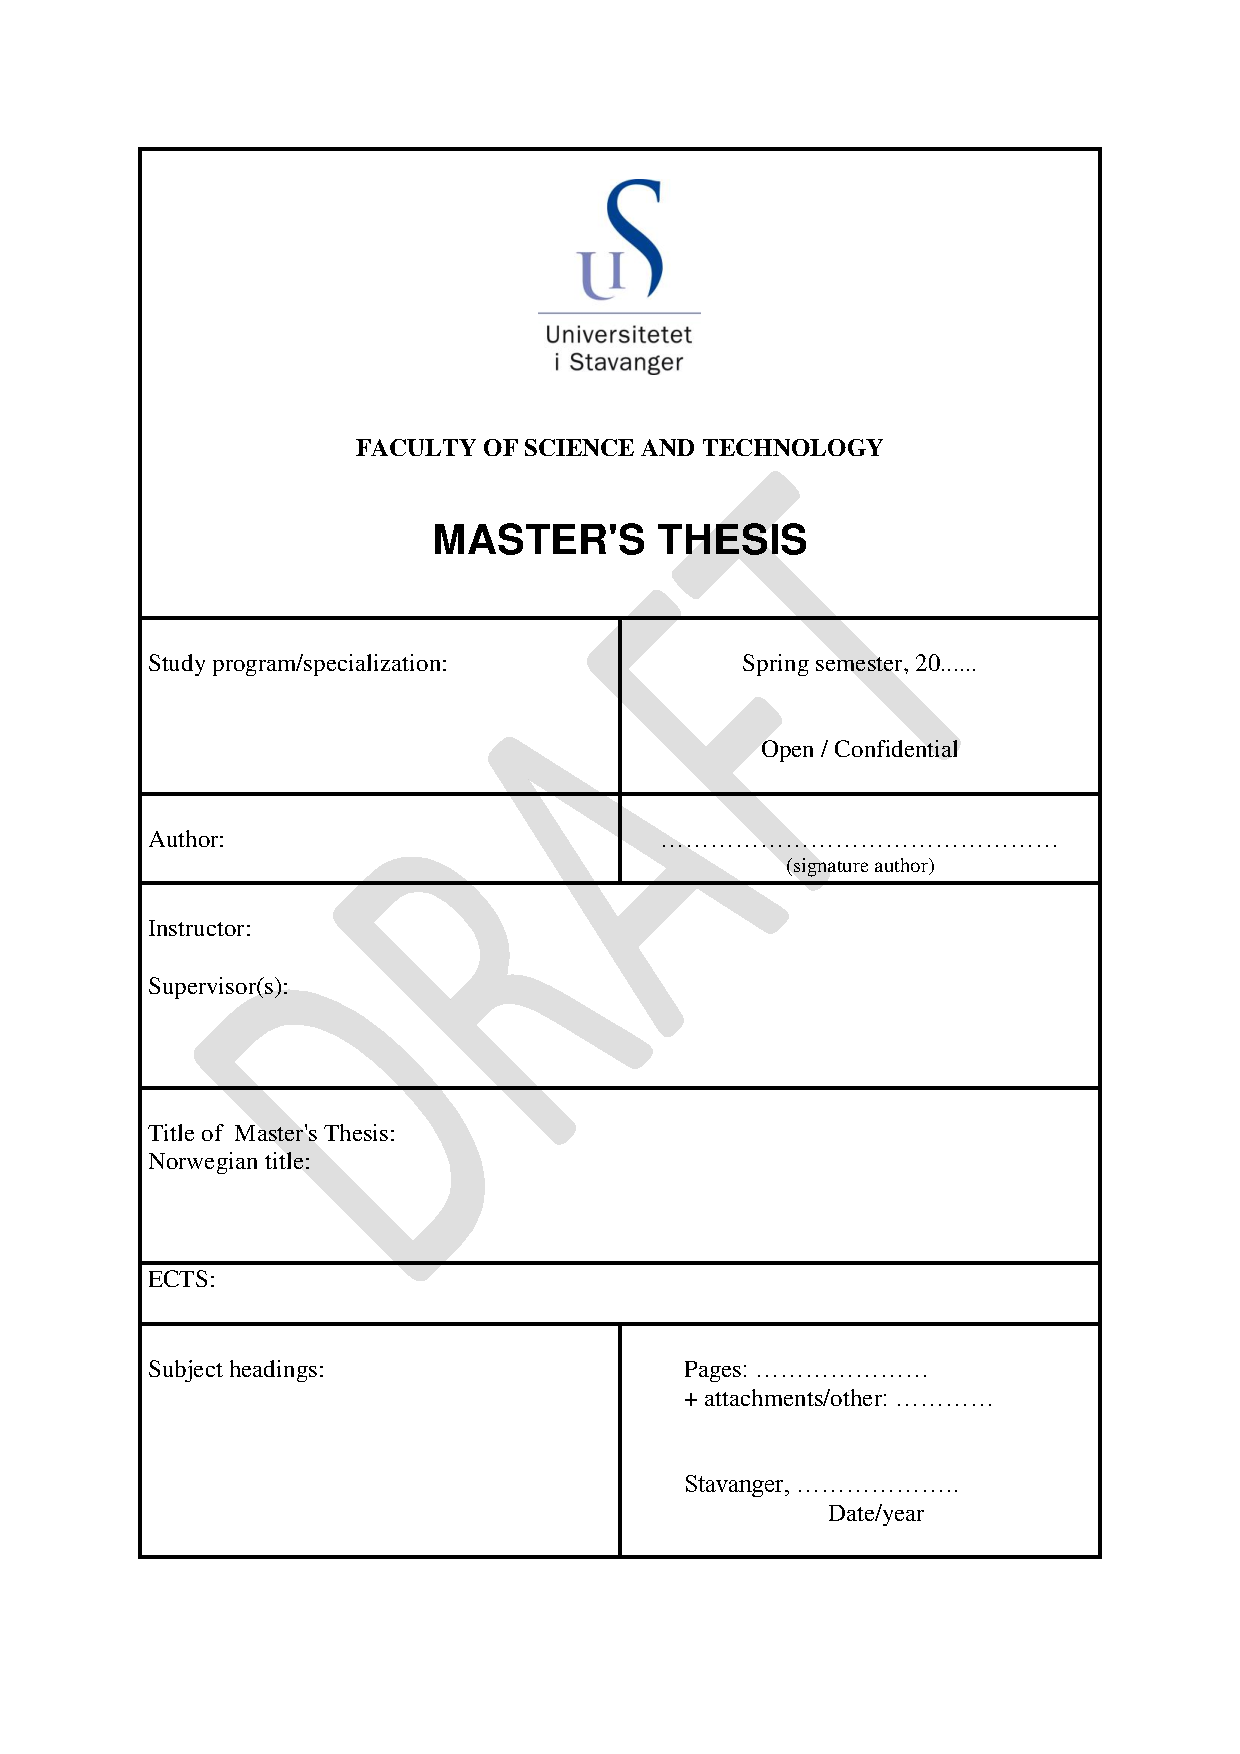
\includepdf[pages={1}]{pdf_pages/draft_front_page.pdf} % REMEMBER TO CREATE CORRECT FRONT PAGE BEFORE SUBMITTING THESIS
    
    % Including personalized front page
    % \thispagestyle{empty}
\vspace*{2cm}
\begin{center}
    %
\includegraphics[width=6cm]{figures/OptiRun.pdf}\\
    \scshape{
        %
\includegraphics[width=6cm]{figures/OptiRun.pdf}\\
        \begin{Huge}\textbf{\scalebox{1}[1.15]{\toolname}}\end{Huge}\\
        \vspace{0.6cm}
        \begin{Large}\scalebox{1}[1.1]{An Approach to Proactive Automated Software Testing}\end{Large}\\
    }
    \vspace{2.6cm}
    %
\includegraphics[width=3cm]{figures/UiS_logo_black}\\
    
\includegraphics[width=3cm]{figures/uis_logo}\\
    \vspace{0.8cm}
    
\includegraphics[width=3cm]{figures/logo_pos_RGB}\\
    \vspace{1.6cm}
    \begin{large}Janicke Falch\\
    \vspace{0.2cm}
    June 2016\end{large}\\
    \vspace{1cm}
    \emph{
        Department of Electrical Engineering and Computer Science\\
        Faculty of Science and Technology\\
        University of Stavangerrrrrrrrrrrrrrrrr
    }
\end{center}
    \vspace*{-1cm}
\section*{\hfill OptiRun \hfill}
\thispagestyle{empty}

\begin{center}
    %
\includegraphics[width=6cm]{figures/OptiRun.pdf}\\
    \scshape{
        \vspace{-1cm}
        \begin{Large}\scalebox{1}[1.05]{A Platform for Optimized Test Execution}\end{Large}\\
        \vspace{0.2cm}
        \begin{Large}\scalebox{1}[1.05]{in Distributed Environments}\end{Large}\\
    }
    \vspace{2cm}
    %
\includegraphics[width=3cm]{figures/UiS_logo_black}\\
    
\includegraphics[width=3cm]{figures/uis_logo}\\
    \vspace{0.8cm}
    
\includegraphics[width=3cm]{figures/logo_pos_RGB}\\
    \vspace{2cm}
    \begin{large}Janicke Falch\\
    \vspace{0.2cm}
    June 2016\end{large}\\
    \vspace{1.6cm}
    \emph{
        Department of Electrical Engineering and Computer Science\\
        Faculty of Science and Technology\\
        University of Stavanger
    }
\end{center}
    
    % Setting page before thesis begins in roman numerals 
    \pagenumbering{roman}			
    
    % Adjusting counter after inserting frontpage
    \setcounter{page}{3}
    \setcounter{page}{1}
    
    % Inserting abstract and acknowledgements
    
    
    \renewcommand{\abstractname}{}
\thispagestyle{empty}
\vspace*{1cm}
\section*{\hfill Abstract \hfill}
\begin{abstract}

\improvement[inline]{TODO}

\comment{
    \noindent
    \textbf{Blind-text} \blindtext \blindtext
    
    \iffalse
        This thesis presents an approach to proactive software testing using scheduled regression tests with rapid feedback.
    \fi
}

\end{abstract}
    \renewcommand{\abstractname}{}
\thispagestyle{empty}
\vspace*{1cm}
\section*{\hfill Acknowledgements \hfill}
\begin{abstract}

\improvement[inline]{TODO}

%\noindent
%\textbf{Blind-text} \blindtext

\comment{
    \noindent
        I would like to express my utmost gratitude to my supervisor Hein Meling, Professor at the Department of Electrical Engineering and Computer Science at the University of Stavanger, for his academic guidance and invaluable feedback throughout my work on this project. I would also like to thank Morten Mossige, [title] at the Department of Electrical Engineering and Computer Science at the University of Stavanger, for [repeated and thorough assistance?].
        \\[7pt]
        \noindent
        Further, I want to thank Kristin Dahle Larsen, Senior IPTV Engineer at Altibox, for her never-ending enthusiasm and for kindly accepting the task of being my external supervisor. % Nevn også Jarle (head of IPTV), head of IPTV (og Marius, IPTV Engineer?)
        \\[7pt]
        \noindent
        Last, but by no means least, I want to offer my sincere thanks to my significant other, Samuel Trevena, for his helping hand in times of need, and for being an excellent resource of moral support and words of encouragement. Thank you for giving me the drive to finish this project!
}    
    
\end{abstract}


% Inserting TOC with custom line spacing (setstretch argument) to avoid odd page breaks
{
    \setstretch{1.2}
    \thispagestyle{plain}
    \tableofcontents
}

\newpage



% Resetting page counter and setting page numbers in thesis in arabic numerals
\setcounter{page}{1}
\pagenumbering{arabic}

% Include chapters
\section{Introduction}
\thispagestyle{plain}
%\thispagestyle{empty}

\comment{"Professional testing of software is an essential task that requires a profound knowledge of testing techniques." (ISTQB Foundations)}

\noindent Software systems, ranging from business applications to consumer products, have grown to form a fundamental element in our society. People are becoming increasingly dependent on computers, and wish to be in control of the digital content they consume. As a consequence of digital content being increasingly accessible, the importance of, and demand for, high-quality software has become substantial. Enhanced pressure on software vendors to deliver frequent releases of high-quality software requires efficiency in every stage of the software development process.

Software testing constitutes a central aspect to the software development process. It plays a critical role in quality assurance and defect detection, and is an important means to ensure that the software in question behaves as expected and according to specifications.

%\cite{http://www.istqb.org/downloads/send/2-foundation-level-documents/3-foundation-level-syllabus-2011.html, pp 11}




\comment{
    Introduction to Software testing in general and then more specifically functional testing, regression testing, web testing - test automation vs manual testing.
    
    Talk a little about Altibox and TV Overalt, their situation (software fuuuulll of bugs, several full time consultants as manual testers), how the author
}

\comment{
    Just a few decades ago, our main source of entertainment in a digital form was television. Today, we use computers, smart TVs, tablets, smart phones and smart watches for active interaction between user and content. We are online and available on multiple platforms at all times, and we expect our software and media content to do the same.
    As an effect of this development, people have grown used to being in control of the software and media content they wish to subject themselves to. Users want constant access to all of their content on every platform, and thus, the demand for high quality software has accelerated rapidly.
}

\subsection{Origin} % Briefly describe why this thesis has been done
Altibox, a subsidiary of the Lyse Group, is a company that provides telecommunication services. They offer a selection of services including broadband, \emph{Internet Protocol Television} (IPTV) and \emph{Voice over Internet Protocol}, (VoIP). Since its origin, the company has grown a great deal, and at a considerably higher pace than originally anticipated. Because the company had trouble keeping up with its rapid development, they neglected to apply a number of established business practices in several different areas, including the field of software testing. \comment{The existing test process will be discussed in Chapter \ref{chapter.discussion}.}

IPTV has long been among Altibox' most prominent services, and has previously been available primarily through the use of TV decoders. In the later years, however, an important focus area for Altibox has been to expand the availability of their TV and \emph{Video On Demand} (VOD) content by applying \emph{Over-The-Top} (OTT) technology, which means that the content is made accessible over the Internet. This is accomplished through the development of \emph{TV Overalt}, which is available both as a web application for desktops and as mobile applications for portable devices.

\subsection{Motivation} % Briefly describe why this thesis has been done
Altibox currently perform all software testing manually. For quite some time, Altibox has wanted to automate some of the tests that are conducted manually on the web-based version of TV Overalt, but have failed to make it a priority. Since user-level tests generally are time consuming, Altibox needed a system that would let them execute such tests efficiently. They also wanted the tests to be executed in a controlled environment.

This thesis presents \toolname; a tool that will help Altibox incorporate test automation according to their needs. The tool is not limited to TV Overalt, however, as it can be applied as a testing platform for a broad range of web applications.

\comment{
FÅ FRAM AT HASTIGHET ER DET ALTIBOX TRENGER ALLER MEST. DE TRENGER AT DE RIKTIGE TEST CASENE BLIR KJØRT SÅ TIDLIG SOM MULIG I EN TEST RUN (within a reasonable amount of time, PRIORITY/BUSINESS IMPACT, ETC.), AT TEST RUNS GENERELT GÅR SUPERKJAPT (DERAV SCHEDULING ALGORITME), OG AT MAN FÅR SVAR ASAP (DJANGO-LOGG, JIRA ISSUES OG MOBILNOTIFIKASJONER)
}
\comment{
Altibox tjenesteleverandør telecommunication (leverer tjenester som internett, telefoni, tv over 400.000 kunder, datterselskap i Lyse-konsernet. 


TV Overalt [...], 

- vokst så raskt at man ikke har etablert prosesser man burde i samme tempo som andre bedrifter (test og andre prosesser), veien blir til når du går, ting skjer fort (mangel på tid, ressurser, kunnskap, kompetanse), konsulenter, eksterne folk -> mangel på etablerte testprosesser ble synlig
- dårlig /ingen testprosess
- knowit sitter i bergen, klager litt på testere fordi det er "plagsomt"

- ott (internet) is the future -> stb er ikke fremtiden, web tar over
når du vil, hvor du vil, på hvilken device du vil - live tv-sendinger er på vei til å dø ut, kundenes forventniger over.  lokal lagring på fysisk disk er på vei ut - cloud is the future
fremtidsrettet
-konvergens mellom gammel type stb og tv overalt, bli mer og mer samme tjeneste
- konsumere innholdet
pvr
}

\subsection{Purpose} % Briefly describe what you wish to accomplish with this thesis / problem statement
The aim of this project was to design and create a tool that would substantiate test automation with the intent to optimize the time of test runs, as well as provide control and feedback of test results. The tool is intended to be utilized during system or acceptance testing, primarily by technical testers.

The main area of use is execution of Selenium test scripts for web applications. Tests should be able to be executed remotely in a controlled distributed environment. A major objective has been the design and implementation of \emph{OptiX}; a mechanism for allocating test cases to available machines in the distributed environment in such a way that the overall execution time of a test set is attempted minimized. Further, an interface for uploading, managing, executing and scheduling test scripts should be included, and logs from results of previous test runs should be made available. Upon a failed test, an option to report this in the issue tracking system used by Altibox, JIRA \cite{jira}, should be provided.

\comment{
    \begin{itemize}
        \item Scheduling of future runs of Selenium test scripts for web applications should be supported.
        \item 
        \item 
        \item 
        \item Information about test scripts, test schedules and execution logs should be stored in a database.
        \item 
        \item A mobile application for receiving notifications upon a failed test should be created.
\end{itemize}
}

\subsection{Outline}

The remainder of this thesis is organized as follows:

\begin{Description}
  \item[\betterfakesc{Chapter} \ref{chapter.background}]\indent provides a theoretical basis for the thesis by discussing some background information relevant to this thesis.
  \item[\betterfakesc{Chapter} \ref{chapter.technology}]introduces some essential tools and technology used throughout this project.
  \item[\betterfakesc{Chapter} \ref{chapter.system_overview}]presents an overview of \toolname, and presents the dashboard from the user's perspective.
  \item[\betterfakesc{Chapter} \ref{chapter.implementation}]describes the implementation of the system. Some features are explained in detail.
  \item[\betterfakesc{Chapter} \ref{chapter.discussion}]presents and discusses some experimental results and evaluates the system.
    \item[\betterfakesc{Chapter} \ref{chapters.further_work}]provides some suggestions for further work.
  \item[\betterfakesc{Chapter} \ref{chapters.conclusion}]concludes this thesis.
\end{Description}
\section{Background}\label{chapter.background}
\thispagestyle{plain}
Before moving onto the technical substance, it will be beneficial to acquire a theoretical basis on the subject of this thesis. This chapter introduces software testing and explains some essential concepts. Further, it presents constraint programming and optimization as well as some previous work related to this thesis.

\subsection{Software Testing}

A fundamental understanding of software testing is a useful prerequisite in order to fully understand the context of this thesis. Consequently, this section provides a short introduction to software testing. Since this is a large field, only a small selection of relevant concepts and ideas will be presented. \comment{The testing strategy, process and technique used in this project will also be introduced here.} % and maybe test policy?

Software testing is the process of evaluating the quality of the application, system or component being tested, commonly referred to as the test object or the system under test. Software testing may involve any action oriented toward assessing the software with the goal of determining whether it meets the required results  \cite{[http://istqbexamcertification.com/what-is-a-software-testing/]}.

Software is developed by human beings who can make errors. These errors may cause defects in the source code. Executing defected code can lead to failure in the program  \cite{http://www.istqb.org/downloads/send/2-foundation-level-documents/3-foundation-level-syllabus-2011.html}. One of the purposes of software testing is to examine the test object with the intent of revealing such defects. Other objectives include to measure and ensure quality, and to provide confidence in the product \cite{SoftwareTestingFoundations}.

\subsubsection{The V-Model}

\begin{figure}[h]
    \centering
    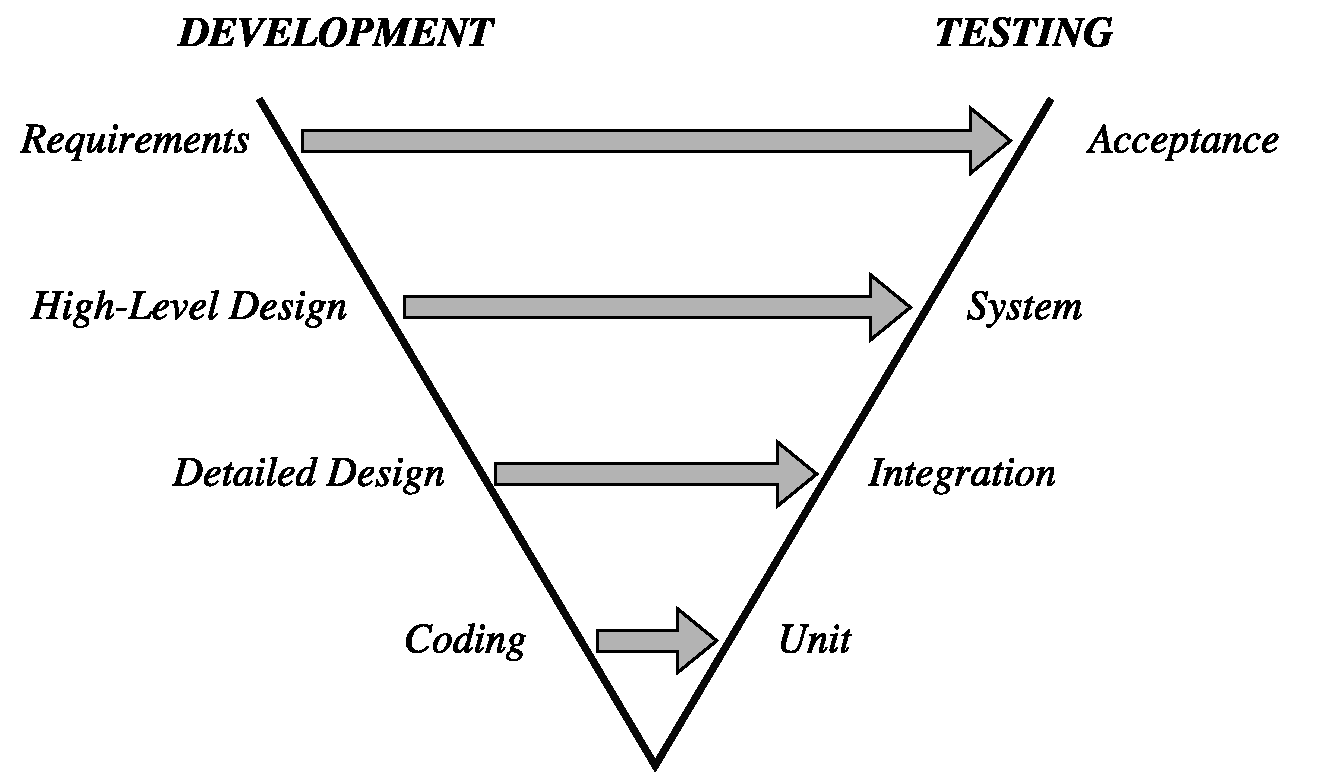
\includegraphics[width=\textwidth]{figures/new/v_model.pdf}
    \caption{The V-Model}
    \label{fig.v-model}
\end{figure}


\noindent The \emph{V-model} is an important asset in software testing, behind which the central idea is to illustrate how each development task in a software development process have a corresponding testing task of equal importance. This is symbolized by the two branches of the letter "V" in the model. The development process is represented by the left branch, which shows the system being gradually developed. The testing process is represented by the right branch, which shows how elements assembled to form progressively larger subsystems are tested \cite{SoftwareTestingFoundations}.

Depending on the literary source, the V-model covers a varying number of levels. The V-model shown in Figure \ref{fig.v-model} is created using the same four levels as found in \cite{systematicSoftwareTesting}. The highest development level covers the gathering, specification and approval of requirements. Acceptance testing correspondingly checks if these requirements are met. Further, high-level design covers the functional design of the system, and corresponds to system testing, which aims to verify if the system as a whole meets the required results. Detailed design covers technical system design and component specification, and integration testing correspondingly verifies that the different components work together as specified. The lowest level is the coding in which the specified components (modules, units and classes) are implemented. It corresponds to unit and component testing. The tests at this level aim to verify that system components perform as specified, by testing them in isolation  \cite{SoftwareTestingFoundations}.

\comment{
    \begin{Description}
        \setlength{\itemsep}{1pt}
        \setlength{\parskip}{4pt}
        \setlength{\parsep}{0pt}
        \item[\betterfakesc{Requirements} $\Leftrightarrow$ \betterfakesc{Acceptance Test}]\hfill\\
        The requirements are gathered, specified and approved. Acceptance tests check if the requirements as specified in the contract are met. This is the highest development and test level of Figure \ref{fig.v-model}.
        \item[\betterfakesc{High-Level Design} $\Leftrightarrow$ \betterfakesc{System Test}]\hfill\\
        The functional design of the system is covered here. System testing verifies if the system as a whole meets the specified requirements.
        \item[\betterfakesc{Detailed Design} $\Leftrightarrow$ \betterfakesc{Integration Test}]\hfill\\
        Detailed design covers technical system design and component specification. Integration testing correspondingly verifies that the different components work together as specified.
        \item[\betterfakesc{Coding} $\Leftrightarrow$ \betterfakesc{Unit Test}]\hfill\\
        The specified components (modules, units, classes) are implemented. Component testing and unit testing verifies that system components perform as specified by testing them in isolation. This is the lowest development and test level of Figure \ref{fig.v-model}.
    \end{Description}
}

\toolname \space is a tool for high-level test execution, and can be applied to the two highest test levels of the V-model; system testing and acceptance testing.


\subsubsection{Black-Box \& White-Box Testing}
\noindent Software testing can be divided into \emph{black-box} and \emph{white-box} testing. White-box testing is based on analysis of the internal system structure, and requires knowledge of the source code. In black-box testing, the test object is seen as black box, whose behavior is watched from the outside. The inner structure of the system is either unknown or unconsidered. Test cases are determined from the specifications of the system. 

Black-box testing is predominantly used for higher levels of testing. The test object is accessed through the user interface (UI). Tests are performed from the perspective of an end user, and aim to mimic a human being interacting with the system. Black-box testing includes functional testing, which is used to validate a particular feature for correctness according to the requirements specifications \cite{SoftwareTestingFoundations}.

\toolname \space performs tests by using Selenium to automate web browsers. It executes functional UI tests on full system builds, and run without access or consideration to the source code and the internal system structure. The test method covered by \toolname \space is therefore black-box testing.



\comment{
    [CI - \url{http://stackoverflow.com/questions/17719385/how-to-make-jenkins-run-selenium-webdriver-testng-java-tests-automatically-on-de}]
}

\subsubsection{Test Automation}
As opposed to humans performing software tests manually, test automation is the practice of writing scripts that conduct tests when executed. Automation can be applied to tests at any level. Low-level tests, such as unit and component tests, generally run fast and are durable since they are isolated from changes in other parts of the system. As we move up to the integration level, the tests does not run as fast, and become less durable since they depend on multiple components working together in subsystems. \toolname \space is concerned with testing the system at the perspective of the end user. Such tests require the system to work as a whole, and thus generally run slower and are more brittle \cite{pluralsight_endtoend}, which is why functional UI tests often are the fewest.

\comment{PLURALSIGHT lecture: Automated Testing: End To End}

There are a number of strengths to automated tests. They are superior at verifying logical functionality. They can be executed any number of times, and they run more quickly than a human interacting with the system, thus saving time and reducing effort. Time saved on manual testing can be used to increase the test coverage, which can provide reduced risk and higher software quality. Tests and tasks that would be error prone if done manually and tests that are repeatedly performed are typical subjects for automation \cite{ASTvol3}. This includes regression testing, which is used to verify that defects have not been introduced in a new version of previously tested software \cite{SoftwareTestingFoundations}.

Manual human testing has a number of benefits too. Human testers can identify corner cases and check how the system responds when it is used in manners it is not designed to be used for. They can also evaluate aesthetics and design of the UI as well as the overall user experience. Thus, test automation on the two highest levels in the V-model should not be a complete replacement for manual human testing; the two should instead complement each other.

Test automation is often incorporated in \emph{continuous integration} (CI) \cite{ci} environments. This has not been done in this project, but is presented in Subsection \ref{furtherwork.ci} as a suggestion for further work.

\comment{
[What should be automated? What can't be obtained through automated testing?] While automated tests may run quickly and effectively, can be cost-effective and are useful for repeating tests the same way repeatedly, the natural exploration that occurs when humans perform manual testing does not happen through executing automated test scripts. Writing and maintaining test scripts are time-consuming, so it is important to only use resources on automating test cases of value.  Test automation should not replace manual testing as a whole; the two should complement each other through a combination of adequate amounts of both manual and automated testing.
}

\comment{
    "Selenium tests run on a real browser, they need to perform actual browser operations and often wait for an HTTP server to respond. The implication is that if you include Selenium tests as part of your build, the build will take much longer to run - so that if currently you’re running a build on every commit, or several times a day, you may have to resort to running the build overnight, and you might need to upgrade your Jenkins workstation or even add more machines to your Jenkins cluster."
}

\comment{
    IEEE/ISO Standard
    ISTQB Websiden (terminologi etc.)
    Software Testing boken
    
    * Se på test nivåer - må forklare på hvilket nivå disse testene utføres.
    * Se på test tilnæringer - f.ekx. black, white, grey box testing eller context driven testing. Finnes og andre. Sjekk litteratur. Du driver med black/grey box testing hvis man ser det utfra det perspektivet.
    * Se på forskjellige test teknikker/metoder - statisk testing, dynamisk testing, funksjonell vs. icke-funksjonell testing etc.
    * Teststrategi, -policy og -prosess -- input fra Alitbox. Spør hva de har for dokumentasjon rundt dette. Ellers finnes dette i IEEE standard. Fornuftig å skrive at du har valgt en strategi, policy og prosess for tid arbeid. Kanskje strategi og prosess er spesielt viktig. Policy er kanskje ikke nødvendig da det ofte er veldig orgranisasjonsspesifikkt.
    
    
    test strategy-A test strategy is an outline that describes the testing approach of the software development cycle.
    test levels - systemtest, integrasjonstest, akseptansetest osv.
    test metode/teknikk - black, white box testing
    test type - 
    
    non-functional testing - the way the system operates.
    functional testing - what the system does
    
    Functional testing is a quality assurance (QA) process[1] and a type of black-box testing 
}

%%% SUBSECTION: Constraint Programming and Optimization %%%
\subsection{Constraint Programming \& Optimization}\label{subsection.cp}
As explained in the previous section, the type of tests targeted in this project are time-consuming. This means that a large collections of test cases, or test sets, could take unnecessarily long time to execute if the tests were not carefully allocated among the available test machines. Minimizing the execution time of a test run has been an important objective in this project.

There are certain requirements that must be fulfilled upon allocating tests in \toolname. A test that is specified to run in a certain browser can only be allocated to a machine with the given browser installed; this is a constraint. \emph{Constraint programming} (CP) revolves around modelling real world constraints by mathematical formalizations, and use them to find feasible solutions to the problem \cite{MortensBok}. 

Some problems have very large sets of possible solutions, while others only have a few or none at all. Sometimes it is not enough to simply find a possible solution to a CP problem, as the quality of different solutions can vary greatly. In such cases, a specification of which solutions are more valuable should be provided to help separate the good solutions from those of poor quality. The objective of the CP problem in this project is to minimize the overall execution time of a test run. An \emph{optimization problem} is a CP problem in which such an objective is specified \cite{MortensBok}.

The optimization problem in this project does not exclusively revolve around finding an optimized allocation - in situations where there are a huge number of solutions to the problem, identifying the best solution can take a vast amount of time. For instance, in a situation with two competing solutions where one provided a 10 second longer overall execution time, but took 20 seconds less to find, this would be the preferred solution. The time it takes to arrive at the solution must therefore also be taken into account. Some stop criteria for searching are defined; these will be presented in Chapter \ref{chapter.implementation}.

Formally, the optimization problem in this project considers a set of tests $\cmsy{T} = \{t_{1},\ \dots,\ t_{n}\}$ with a corresponding set of durations $\cmsy{D} = \{d_{1},\ \dots,\ d_{n}\}$ in which the values are derived from the durations of earlier executions of each test. Further, it considers the current set of available test machines $\cmsy{M} = \{m_{1},\ \dots,\ m_{m}\}$. A pre-processing function $p$ identifies the subset of machines each test can be executed on, and a function $f$ defines the actual allocations with the overall execution time $T_{e}$. The problem seeks to minimize the total time $T_{t}$, which consists of $T_{e}$ plus the searching time it takes to find the solution $T_{s}$. Thus, the expression we wish to minimize is $T_{t} = T_{e} + T_{s}$. Additionally, all tests in the test set must, if possible, be executed exactly once on a machine that fits any specified requirements for browser and operating system.

Furthermore, the following list of assumptions are expected to be strictly imposed:

\begin{Description}
    \item[Non-preemptive execution]- Once a test execution has started, it will run uninterrupted until it completes.
    \item[Non-cumulative execution]- Each test machine can only execute a single test at a time. This could have been implemented differently, but as each test requires a great deal of resources, this would prolong the execution of each test, as well as make the durations more unpredictable.
    \item[Machine-independent execution time]- Although the execution time will not necessarily be machine-independent in reality, depending on machine performance, this is considered an assumption.
\end{Description}

%%% SUBSECTION: Related Work %%%
\subsection{Related Work}
Some work has previously been done on the subject of test case scheduling and automation of functional UI tests for web applications. This section presents the scheduling method \emph{TC-Sched} and the automated testing platform \emph{Sauce Labs}.

\subsubsection{TC-Sched}
TC-Sched is a time-aware method for minimizing the execution time of test cases within a distributed system with resource constraints. Mossige \emph{et al.} proposed the method in \cite{tcsched}. The authors define the \emph{optimal test case scheduling} (OTS) as the optimization problem of finding an execution ordering and assignment of all test cases to machines, in such a way that each test case is executed once, no global resources such as measurement instruments or network devices are used by two test cases at the same time, and the overall test execution time is minimized. TC-Sched addresses situations in which some operations may require exclusive access to one or more global resources, such that only one test case can access each resource at a given time. Including the aspect of global resources in this project would have been redundant as there are no such resources involved.

\subsubsection{Sauce Labs}
Cloud testing services use cloud computing environments as a means of simulating real-life user traffic. Sauce Labs is a cloud-hosted platform for automated testing of web and mobile applications. One of the founders, Jason Huggins, were also the original creator of Selenium \cite{SauceLabsPressCoverage}, which will be introduced in Section \ref{subsec.selenium}.

Sauce Labs bear some similarities and some dissimilarities with the design of \toolname. Both platforms are frameworks for automating UI tests for web applications through execution of Selenium test scripts. They both execute tests remotely in distributed environments using Selenium Grid. However, whereas Sauce Labs perform test execution on virtual machines (VMs) that are created prior to each test run and destroyed immediately after \cite{SauceLabsFeatures}, \toolname \space requires the use of either real, physical machines or customized VMs that remain intact after use. Because of the number of machines in \toolname \space being limited to the machines connected to the distributed system, an algorithm for optimizing the overall execution time of test runs is also needed here. While Sauce Labs executes tests in their own data centers in a remote location and their own environments, \toolname \space performs tests on the test object locally and in an environment intended for testing of the given test object, in this case TV Overalt. Sauce Labs is a paid service for which customers pay to gain access to using a limited number of concurrent virtual machines for a limited amount of time each month. The optimization algorithm in this project also distinguishes the two projects even further.

\comment{
    - TC-sched etc
    - Saucelabs:
        + Similarities: Uses Selenium Grid and Selenium WebDriver(?), supports distributed testing and all other benefits of Selenium+Selenium Grid.
        - Dissimilarities: Runs tests on virtual machines in the cloud; _not_ in a distinguished suitable environment, and _not_ on real, physical machines/devices that we are in complete control over. Does not create tasks in the issue tracker. Maybe: Runs all tests in parallell? And does not (?) provide a OTS/task scheduling algorithm. Costs money: pay a certain amount for accessing a limited number of VMs a limited number of minutes each month. In this solution, you can use real-life physical company owned devices and machines or customized virtual machines as much as desired at anytime.
}
\section{Technology}\label{chapter.technology}
\thispagestyle{plain}
A number of distinctive tools and technologies have been applied throughout the work on this project. This chapter briefly introduces the most essential of these tools and technologies.%The most essential of these tools and technologies will be introduced in this chapter. 

\subsection{The Python Programming Language}
The Python programming language has largely been used in the conduction of this project. Python has efficient high-level data structures, and is known for being simple, yet powerful. Since Python programs are executed by an interpreter, it is considered an interpreted language \cite{abyteofpython}.

Building this project on Python was a natural choice for several reasons. Python is compatible with Selenium, which is introduced in Section \ref{subsec.selenium}. Other reasons include offering a large set of libraries and having high-quality documentation. Additionally, Python supports multithreading and is suitable for running a program as a service. Details of the implementation will be discussed in Chapter \ref{chapter.implementation}. 
\improvement{Will change to Python 3.x if time.} Version 2.7.11 of Python has been used in this project.


\subsection{Selenium}\label{subsec.selenium}
Selenium is an umbrella project for automation of web browsers. Several different tools and libraries are included in the framework, all with the common goal of supporting browser automation. Selenium can be used to automate different types of browser jobs such as web-based administration tasks, but is primarily \comment{most commonly?} used for test automation. The project is released under the Apache 2.0 license and is thus free and open-sourced. Selenium has language bindings for several different programming languages, including Python. The Selenium tools used in this project will be introduced below. %[source]

%%% SUBSUBSECTION: Selenium WebDriver %%%
\subsubsection{Selenium WebDriver}
Selenium WebDriver consists of a set of libraries that helps with automation of tests for web applications, and a set of executable WebDriver files, one for each browser, that perform the actual automation specified in the WebDriver scripts. Selenium WebDriver interacts directly with the browser by sending calls using the native support for automation for each browser \cite{selDocWebDriver}. Selenium WebDriver runs on Windows, Linux and Macintosh, and supports most conventional web browsers, including Firefox, Chrome, Internet Explorer, Opera and Safari.

The WebDriver is used to create a new instance of the requested web browser. It is used to fetch a given web page, and then locates UI elements. When an element is located, the WebDriver can be used to perform an action on the element, such as clicking a button, checking a checkbox, or populating a text field.

\vspace{4mm}
\begin{lstlisting}[caption=Selenium WebDriver Example, label={listing.selWebDriverEx}]
 from selenium import webdriver
    
 # Create a new instance of the Chrome WebDriver
 driverdriver = webdriver.Chrome("<file path>/chromedriver.exe")
  
 # Go to the Altibox TV Overalt start page
 driver.get("https://tvoveraltstg.altibox.no/")
  
 # Locate and click the Login button
 login_button = driver.find_element_by_class_name('btn-login')
 login_button.click()
\end{lstlisting}
\noindent
\lstlistingname \space \ref{listing.selWebDriverEx} shows a simple example of how Selenium WebDriver can be used with Python to open the Chrome web browser, navigate to the Altibox TV Overalt start page, locate the \emph{Login} button, and click it. \toolname \space revolves around executing scripts that uses the Selenium 2.0 libraries and WebDrivers to execute automated web browser tests.

\subsubsection{Selenium Grid}\label{subsubsec.seleniumGrid}
Selenium Grid is a tool for executing Selenium tests on remote machines in a distributed environment, and thus allowing for parallel execution. This also opens up for running tests on different operating systems.

Reasons for wanting to incorporate Selenium Grid include being able to run tests against multiple browsers, browser versions and browsers running on different operating systems, and to reduce the execution time of the tests. In practice, a grid is made up of one Selenium Grid Server; a \emph{hub}, and one or more slave machines; \emph{nodes}, all running a Selenium Standalone Server. The nodes use Selenium WebDriver to communicate with the hub through a JSON wire protocol \cite{selGrid}.

Selenium Grid 2.0 and Selenium Standalone Server 2.51.0 were used in this project.

    \iffalse
        selenium web browser automation (collection of Python libraries)
        selenium server?
        selenium grid
    \fi

\subsection{Django}\label{subsection.django} % Read again towards the end and change the name of the Web interface to something more suitable
Django is a high-level web development framework that is implemented in the Python programming language. It encourages rapid development and enables efficiently maintainable web applications of high quality. The framework is a free and open-sourced project maintained by the non-profit organization \emph{the Django Software Foundation}, who describe the framework as fast, secure and scalable \cite{djangoproject}. Comparable to Selenium, Django is also essentially a collection of Python libraries \cite{thedjangobook}. The Django libraries can be imported and used to implement web applications. Some additional HTML, CSS and JavaScript code has been applied along with the Python code.

\comment{
\emph{Models} play a central role in web applications built on Django. The models are sources of information that contain fields and behaviors of the data being stored. The models define the database layout, and each model typically maps to an individual table in the database, in which instances of the model are later stored \cite{https://docs.djangoproject.com/en/1.9/topics/db/models/}. \lstlistingname \space \ref{listing.djModelEx} shows a simple example of how a model is created in Django.
\vspace{4mm}

\begin{lstlisting}[caption=Django Model Example, label={listing.djModelEx}]
from django.db import models

class Schedule(models.Model):
    title          = models.CharField(max_length=80)
    start_time     = models.DateTimeField()
\end{lstlisting}
\noindent
}

Aside from allowing rapid progression of development, one of the main reasons for choosing Django rather than building the dashboard from scratch or using a different web framework, is its powerful administrator site. An administrator site was exactly what was needed to build the dashboard of \toolname. Another contributing factor was to provide consistency and the ability to communicate seamlessly with the remaining parts of the system, since Django builds on the same programming language as the rest of the system. The dashboard will be presented in Chapter \ref{chapter.system_overview}. Details concerning the implementation will be explained in Chapter \ref{chapter.implementation}. Version 1.9 of Django was used in this project.

\subsection{OR-Tools}\label{subsection.ortools}
Google's \emph{Operations Research Tools} (OR-Tools) \cite{ortools} is an open source library for combinatorial and constraint optimization. The tool set is written in C++, but is available with bindings for other programming languages such as Java, C\# and Python. The OR-Tools library strictly conforms to the Google coding styles, and is of such high quality that it has been accepted for usage internally at Google.

\lstlistingname \space \ref{listing.or_tools} shows how a simple optimization problem is solved using this library. In this problem, a list of integers will be assigned values ranging from 0 to 2. A constraint specifying that no two identical numbers should be placed beside each other is added as a constraint. Maximizing the sum of the integers is specified as the objective. The solver searches for better and better solutions until finally arriving at an optimal solution.

\vspace{4mm}
\begin{lstlisting}[caption=OR-Tool Implementation, label={listing.or_tools}]
from ortools.constraint_solver import pywrapcp

solver = pywrapcp.Solver('')

variables = [solver.IntVar(0, 2) for _ in range(3)]

for i in range(len(variables) - 1):
    solver.Add(variables[i] != variables[i + 1])

db = solver.Phase(variables, solver.CHOOSE_FIRST_UNBOUND, solver.ASSIGN_MAX_VALUE)
objective = solver.Maximize(solver.Sum(variables), 1)
solver.NewSearch(db, objective)

while solver.NextSolution():
    result = [int(item.Value()) for item in variables]
    print result, "Sum =", sum(result)

>>> [0, 2, 0] Sum = 2
>>> [0, 2, 1] Sum = 3
>>> [1, 2, 1] Sum = 4
>>> [2, 1, 2] Sum = 5
\end{lstlisting}

As a means to evaluate the optimization mechanism of test allocations designed for this project, an alternative version using OR-Tools has also been implemented. This alternative implementation, as well as a discussion, evaluation and thorough comparison of the two versions will be presented later in the report.
\section{System Overview}\label{chapter.system_overview}
\thispagestyle{plain}

This chapter aims to provide an overview of how \toolname \space is assembled by describing the design and architecture of the system. System setup will be described thereafter, followed by a presentation of the web-based user interface.


\comment{
\info[inline]{[Frontend/On-Stage]

Detailed description of what the system does and how it works from the perspective of the user. Use edited screenshots with extra info and markings.

Don't add screenshots until the product is finished. This chapter should be around 10 pages or a little more (with screenshots)?}}





%%%%%%%%%%%%%%%%%%%%%%%%%%%%%%%%
% SUBSECTION: Architecture
%%%%%%%%%%%%%%%%%%%%%%%%%%%%%%%%
\subsection{Architecture}

\comment{\improvement[inline]{Chart of system architecture? Yes.\\ Chart of data flow? Maybe? (Or next ch.)\\ Explain how components communicate? Or should that be in next chapter? *confused*}}

\begin{figure}[p]
    \centering
    \thisfloatpagestyle{empty}
    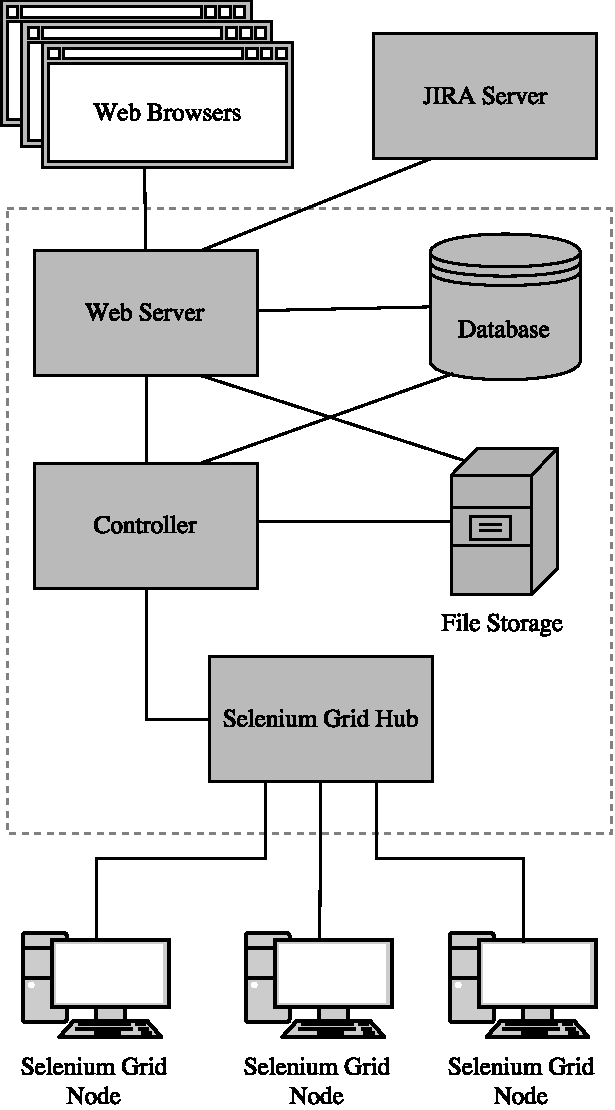
\includegraphics[height=\textheight]{figures/architecture4.pdf}
    \caption{System Architecture}
    \label{fig.architecture}
\end{figure}

\toolname \space is operated through a web-based dashboard. This web service works as a content management system for test scripts. It also allows for sending test execution requests for the available test scripts and for scheduling test runs ahead of time. 

Figure \ref{fig.architecture} shows the structural architecture of the system. In this case, the web server, the controller, the database, the file storage and the Selenium Grid Hub are all located on the same machine, hence the dashed border around these elements in the figure. They could, however, be separated with little effort if needed.

The web server uploads test scripts to a file location on the server. Meta data about the test cases as well as other information such as test groups, planned test executions, test results and user authentication, including credentials and permissions, are also stored in the database. The web server can report defects in the issue tracker system, for which Altibox uses JIRA.

The controller listens to test execution requests triggered through the dashboard, and checks the schedule. Upon a pending execution, it fetches the given test script from the file storage. Test scripts are sent to the current instance of the Selenium Grid Hub with specifications of which node in the grid that the test script should be executed on. The hub then triggers the given node to execute the test. After the test has finished, the controller stores the result in the database.







%%%%%%%%%%%%%%%%%%%%%%%%%%%%%%%%
% SUBSECTION: Setup
%%%%%%%%%%%%%%%%%%%%%%%%%%%%%%%%
\comment{
\subsection{Setup}
\improvement[inline]{TODO}
\comment{\improvement[inline]{Explain how to set up the system?}
\info[inline]{Add a some customized VM ISO images to the thesis submission, each with different browsers installed. Preferably include a OSx VM. This subsection walks through how to set up the environment and start everything that needs to be started.}}
}








%%%%%%%%%%%%%%%%%%%%%%%%%%%%%%%%
% SUBSECTION: Dashboard
%%%%%%%%%%%%%%%%%%%%%%%%%%%%%%%%
\subsection{Dashboard}
The graphical user interface of \toolname \space is web-based, and is built on the high-level Web framework Django. The framework provides a powerful automatic administrator interface, which has been used as a foundation for the development of the dashboard. Working with Django thus allowed for rapid development while retaining control of the content and functionality of the website.

This section presents the dashboard from the user's perspective. An in-depth presentation of how some of the functionality has been implemented can be found in Chapter \ref{chapter.implementation}.

\comment{
\info[inline]{General explanation of how django change lists work? How attributes are chosen for listing, searching, filtering, that they are sortable. How object history works. Nah, maybe move that to implementation?}
}




%%%%%%%%%%%%
% SUBSUBSECTION: Home Screen
%%%%%%%%%%%%
\subsubsection{Home Screen}

\comment{\info[inline]{}}

\begin{figure}[h]
    \centering
    
\includegraphics[width=\textwidth]{figures/placeholder.png}
    \caption{Home Screen}
    \label{fig.home}
\end{figure}
\noindent
After logging in, the home screen is the first thing that meets the eye of the user. This screen provides navigation to all of the modules and pages described subsequently. In order to give the user an indication of status, some graphs that show the results of recent test runs, as well as key performance indicators and other important information is displayed on this page.


%%%%%%%%%%%%
% SUBSUBSECTION: Authentication and Authorization
%%%%%%%%%%%%
\subsubsection{Authentication \& Authorization}

\comment{
\unsure[inline]{Some gamification element might be added, in which case this module must be customized, and screenshots must be provided.}
}

\begin{figure}[h]
    \centering
    
\includegraphics[width=\textwidth]{figures/placeholder.png}
    \caption{Authentication and Authorization Module}
    \label{fig.tc_mod}
\end{figure}

\noindent The Django administrator interface provides some built-in functionality, including a module for authentication and authorization of users. \emph{Superusers} can list, edit and create new user accounts. They can also change user info and the permissions of other user accounts, add them to user groups, and specify the permissions of user accounts.

\toolname \space is a tool that is meant to be part of a business process in which only trusted peers should be allowed to take part, and by extension, \toolname \space should only be operated by trusted associates. For this reason, no user accounts can be created by anyone other than a superuser. Thus, any person who wants and account must request this by someone with superuser privileges. 

By default, all passwords are encrypted by Django before being stored in the database.






%%%%%%%%%%%%
% SUBSUBSECTION: Test Case Module
%%%%%%%%%%%%
\subsubsection{Test Case Module}\label{subsubsection.test_case_module}

\begin{figure}[h]
    \centering
    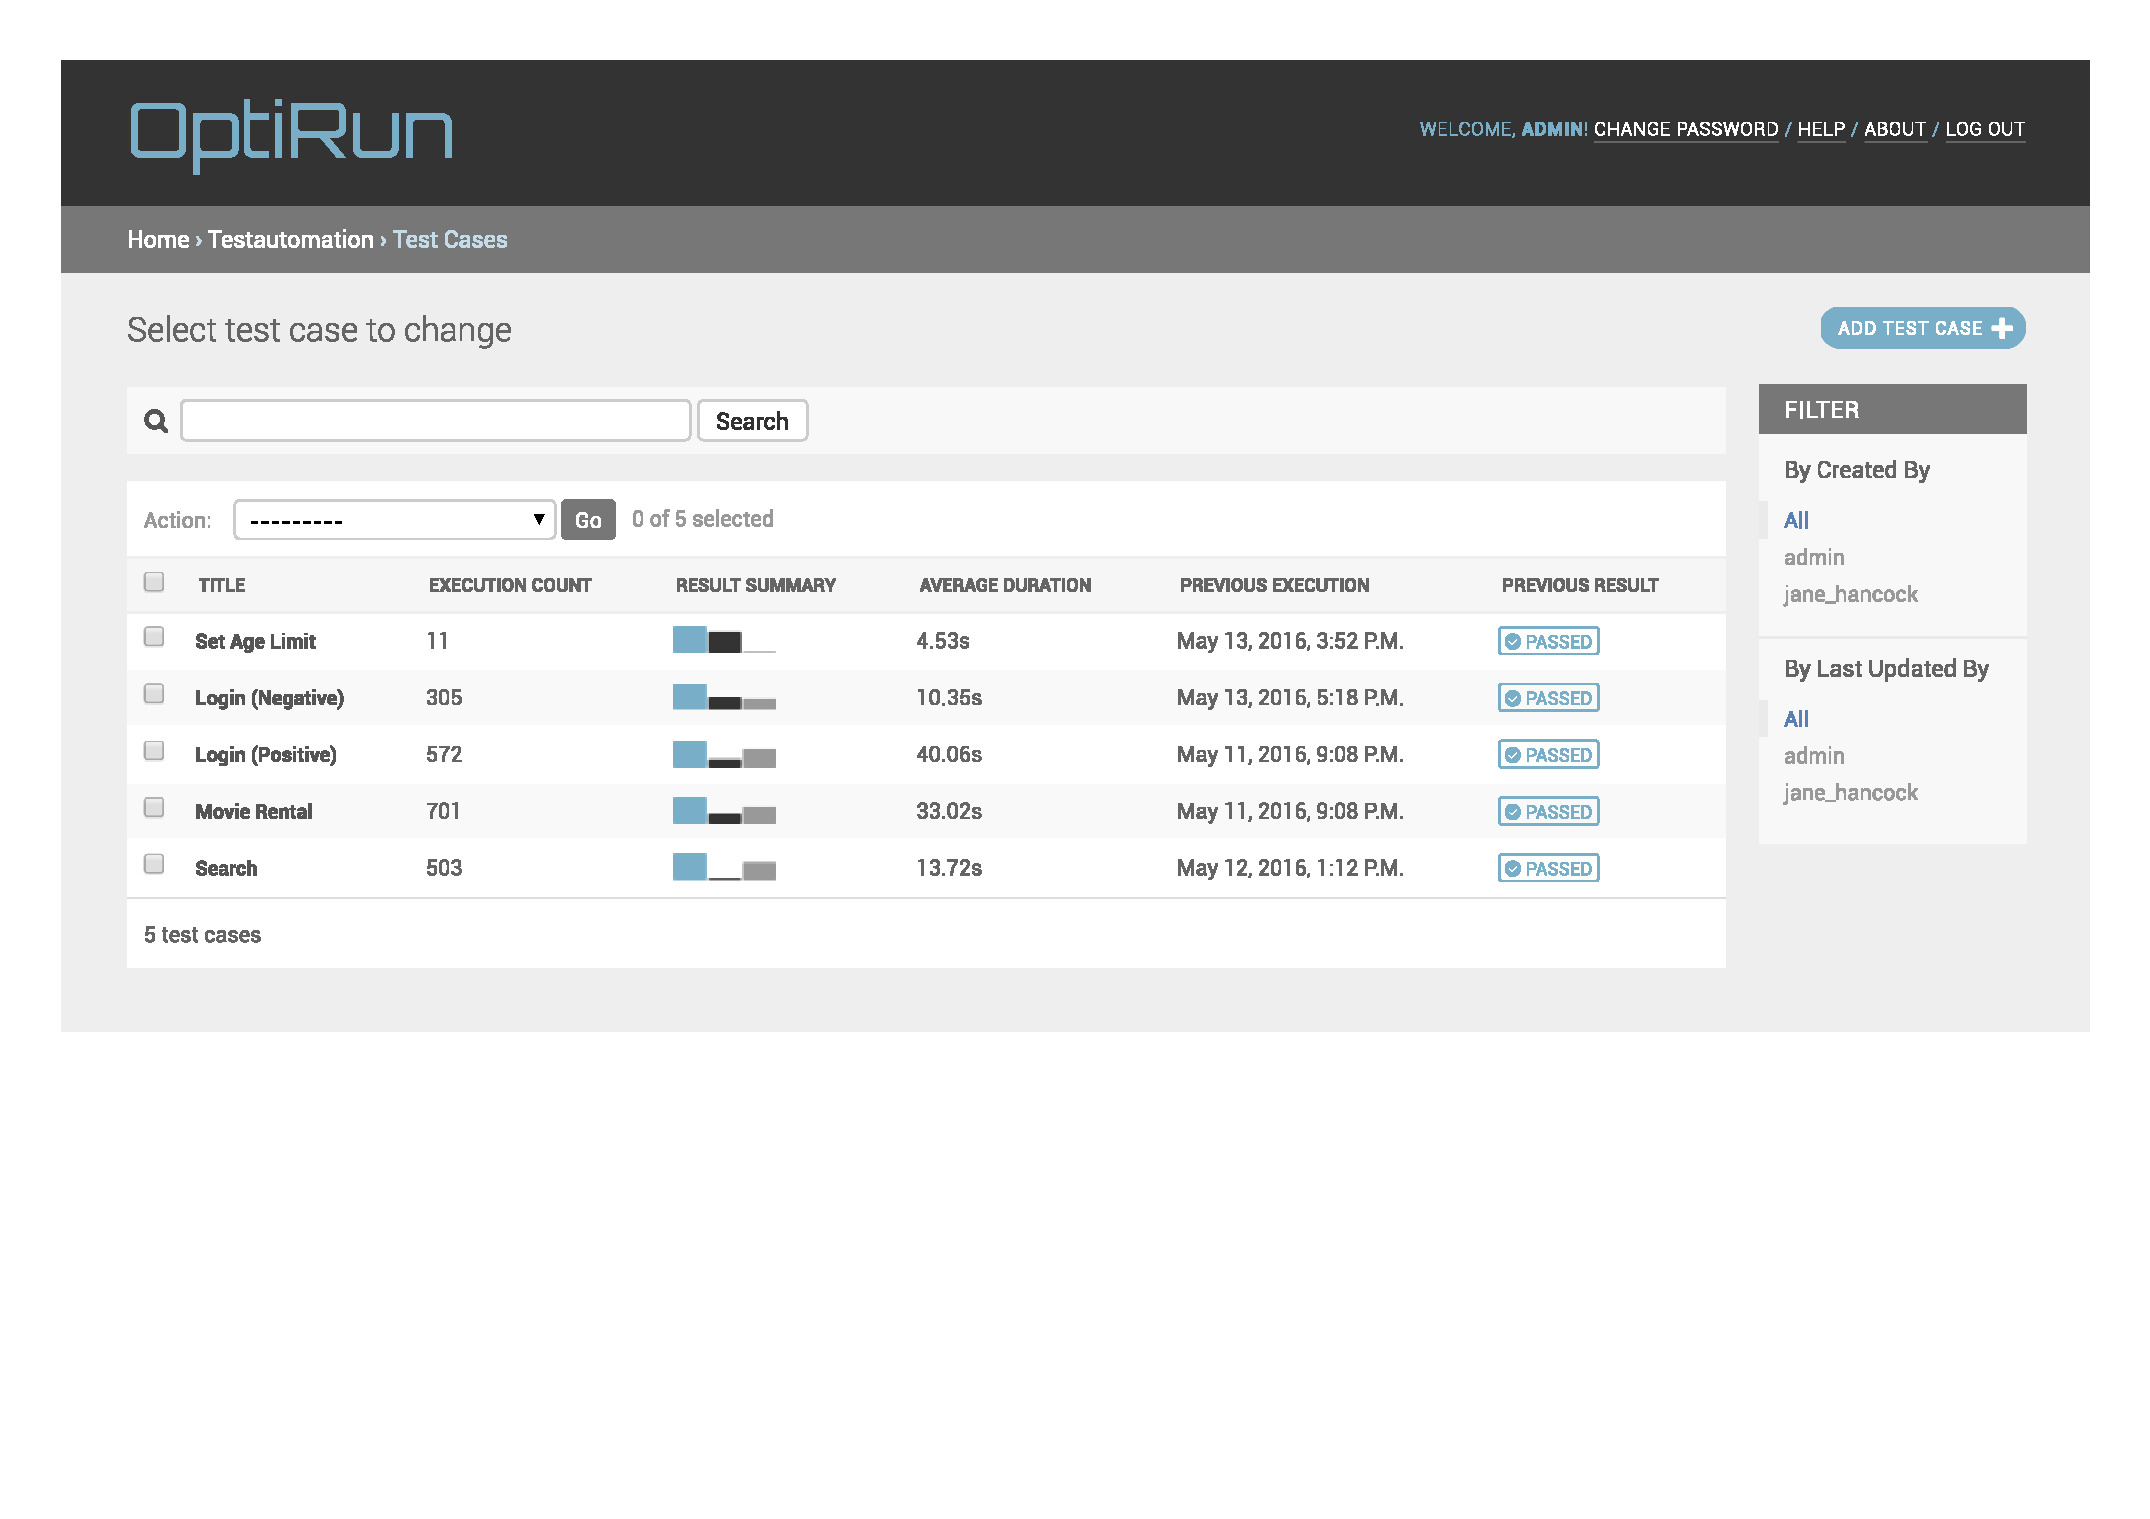
\includegraphics[width=\textwidth]{figures/test_cases.pdf}
    \caption{Test Case Module}
    \label{fig.tc_mod}
\end{figure}

All registered test cases are listed in this module. The list contains meta data about the test cases as well as some values that are retrieved or calculated using information from other tables in the database. This includes the number of times the test case has been executed, the average execution time, the result of the previous execution and when the test case was last executed. It is possible to search and filter the list to narrow down the elements listed, and to sort the list by clicking on the attribute names in the table header.

New test cases can be created by clicking the button labeled \emph{Add Test Case} in the upper right of the view. This opens a new page with a form in which the test script can be uploaded and corresponding details about the test case can be filled in. Which groups the test case should be a member of can also be specified here. Test cases can be members of multiple groups, or none. After a test case has been created, it can be edited by clicking on the title of the test case in the test case list.

It is possible to select test cases and perform actions on them. The action options - \emph{Delete selected test cases} and \emph{Execute selected test cases} - are located in a dropdown menu above the test case list. The former is a built-in Django function which, after the user confirms deletion in and intermediate page, removes all meta data regarding the selected items from the database. The \emph{Execute selected test cases} action is implemented for \toolname. The action takes the user to an intermediate page in which they can specify the platform and browsers the test cases should be executed on.

After an action has been attempted performed, a feedback message stating whether the action was successful is displayed on the screen.

\comment{
\info[inline]{js must be extended to check which browsers/platforms are currently available and update each time a browser/platform is selected. Form validation must also be included (check if all platform/browser combinations are still available when Execute is pushed).}
}

\begin{figure}[h]
    \centering
    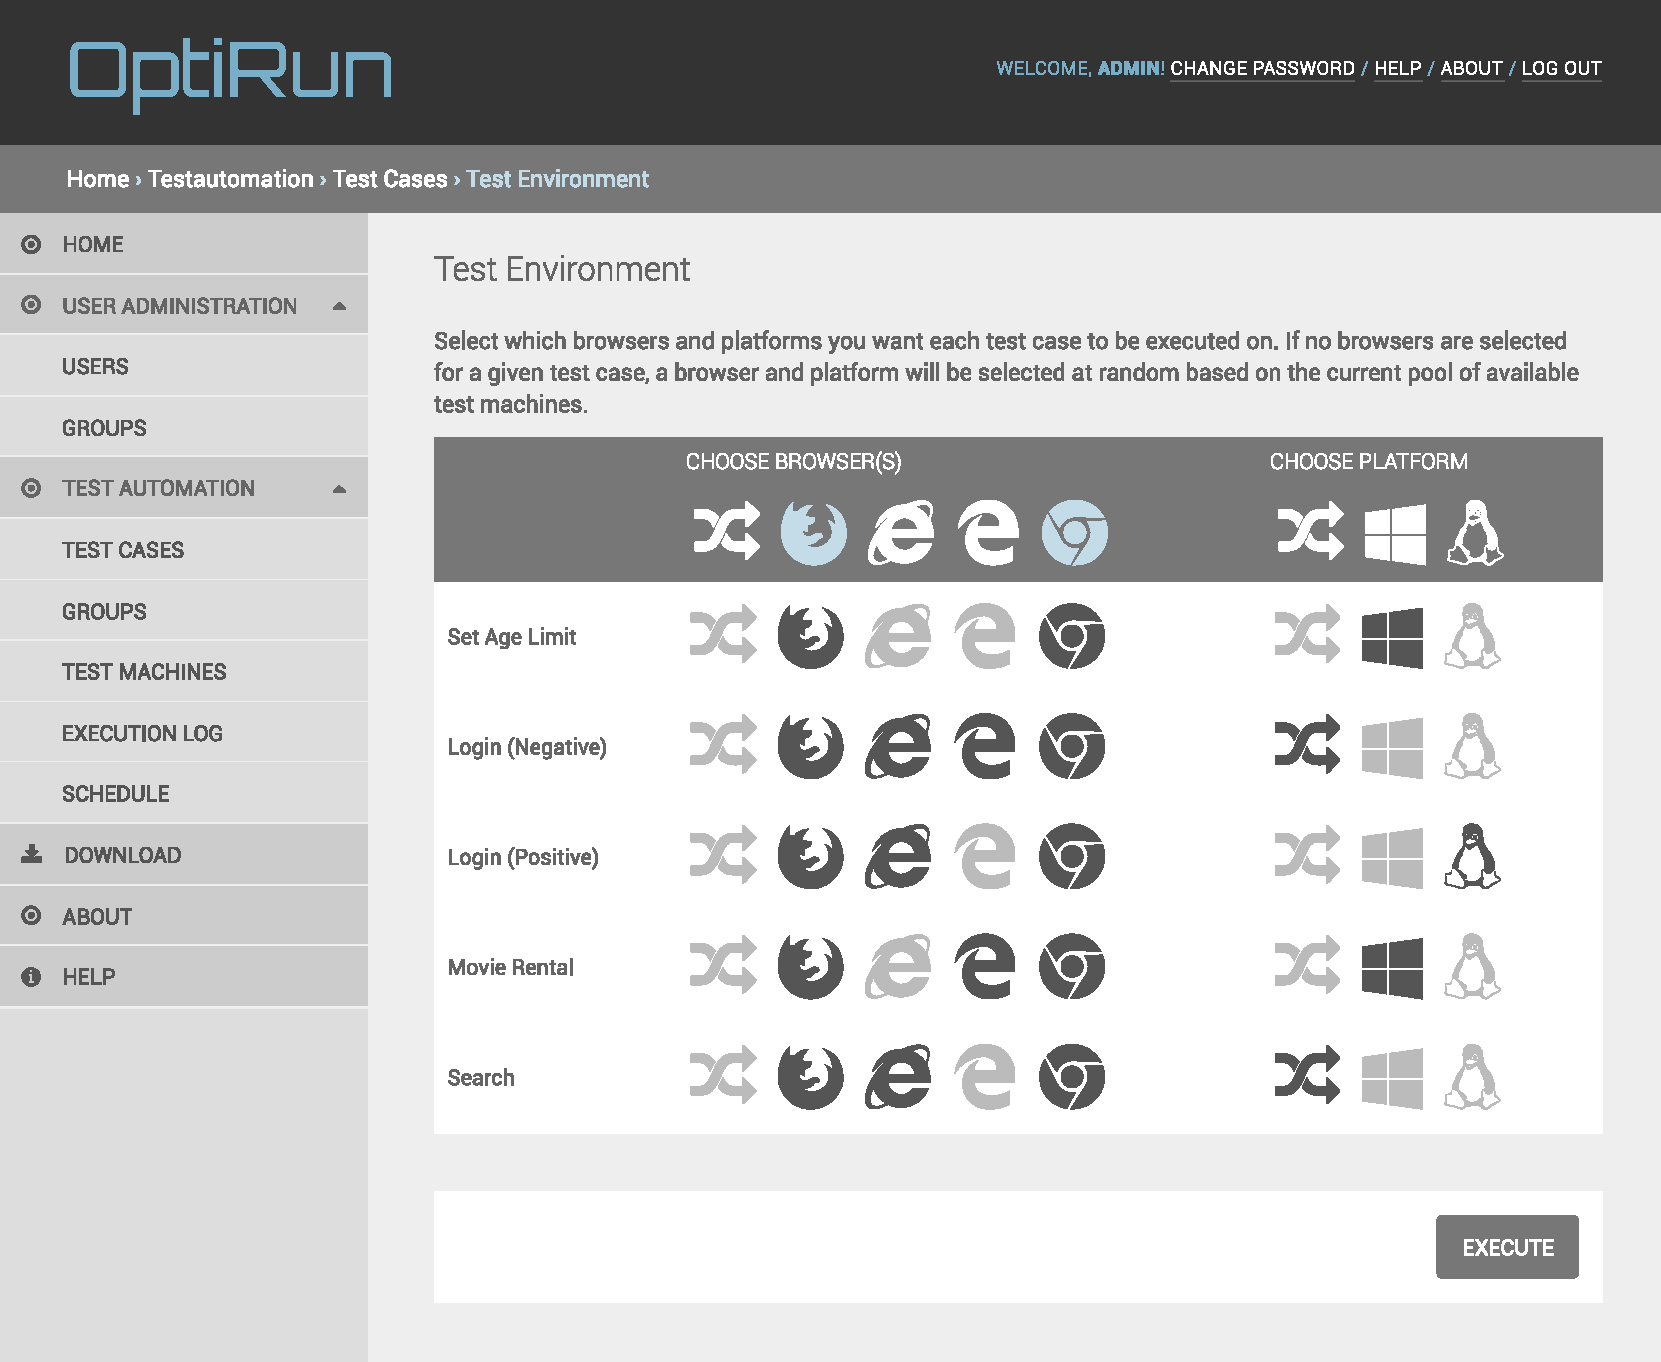
\includegraphics[width=\textwidth]{figures/screenshots/OptiRun_immediate_test_execution_intermediate.pdf}
    \caption{Intermediate Page for Immediate Test Execution Requests}
    \label{fig.tc_intermediate}
\end{figure}

\subsubsection{Test Group Module}

Test groups are listed similarly to test cases as described in Section \ref{subsubsection.test_case_module}. As with the test cases, group items can also be searched, filtered and sorted. Additionally, new groups can be created, and existing groups can be edited.

However, the group model is simpler than the test case model. The purpose of this model is to group together test cases that are often executed in the same test run, such as tests revolving around the same functionality in the test object.

\subsubsection{Scheduling Module}

The scheduling module provides an interface for planning test runs in the future. As with the test cases and groups, schedules are also displayed in a list can be searched, filtered and sorted. Schedule objects can be created and changed. Additionally, the schedule list enables schedule objects to be activated and deactivated from the action menu. Only activated schedule objects will start test runs according to their specified time of execution.

\begin{figure}[h]
    \centering
    
\includegraphics[width=\textwidth]{figures/placeholder.png}
    \caption{Schedule Creation Form}
    \label{fig.sched_mod}
\end{figure}

Upon creating or editing a schedule object, an execution time can be specified along with any desired recurrence pattern along with the option of providing an end time. Test groups or individual test cases that should be included in the schedule object are also specified here.

\subsubsection{Execution Log}

The layout of the log is the same as the remaining list views, but the functionality differs in that log items can not be edited. Log items are created and inserted into the database based on the result from test executions. Each log object corresponds to an execution of an individual test script. The information listed in the logs include a number of attributes such as the duration of the test execution, the IP address or hostname of the machine on which it was executed, as well as information such as browser, platform and test result. Additionally, the content from the standardized data streams \emph{standard error} (stderr) and \emph{standard output} (stdout) are also included. Stderr typically streams any automatically generated error messages or diagnostics from command line programs \cite{http://www.linfo.org/standard_error.html}, while stdout consists of the output data from the programs themselves (if any) \cite{http://www.linfo.org/standard_output.html}, using the \emph{print} command in Python scripts. For better human readability, the fields are labeled \emph{Console Log} and \emph{Output} respectively. Figure \ref{fig.log} shows a detail view of a log object.

\begin{figure}[h]
    \centering
    
\includegraphics[width=\textwidth]{figures/placeholder.png}
    \caption{Execution Log Detail View}
    \label{fig.log}
\end{figure}

Failed test executions can be reported to JIRA. This is done by marking the log items that should be reported and selecting \emph{Report to JIRA} from the actions menu. When clicking on a log item to view details about the execution, there is also an attribute displaying any existing JIRA issues reported by \toolname \space for the specific test, with links to the URL of the specific JIRA issues.







\subsubsection{Other}

\comment{\todo[inline]{TODO}}

\comment{\info[inline]{These pages contain how tos, different explanations of stuffs, where to find whatever, how to set up everything. About contains any necessary licenses (orbitron font, icons, etc.) and any other info about \toolname \space and maybe that it was lovingly created by me as my master's thesis?}}

In addition to the content that has already been introduced, \toolname \space also includes the following static pages:

\begin{Description}
    \item [Download] Test machine packages for Linux and Windows can be downloaded from this page as well as a test script template that needs to be used with \toolname.
    \item [Help] This page contains information regarding how \toolname \space works, how to set it up and how to use it. This page can be of help to technical testers who wants to use the tool, and otherwise to those who wants additional insight into how it works.
    \item [About] This page provides a presentation of what \toolname \space is and how it came to be. Necessary licenses are also included in this page.
\end{Description}
\section{Design \& Implementation}\label{chapter.implementation}
\thispagestyle{plain}

\comment{[Backend/Off-Stage]}

This chapter aims to explain how \toolname \space is designed and implemented. \comment{It starts with a visualization and narrative of how data flows through the system.} It \comment{then} provides a description of how the system utilizes Selenium Grid. The implementation of the controller and some important details about this part of the system will then be presented. Further, the test allocation mechanism called \emph{Opti-X} will be explained with an accompanying example to illustrate how the mechanism works step-by-step will be presented. The chapter then explains how the database is structured in addition to the how it is accessed using Django libraries, before finally presenting some important implementation details about the dashboard.



%%%%%%%%%%%%%%%%%%%%%%%%%%%%%%%%
% SUBSECTION: Data Flow
%%%%%%%%%%%%%%%%%%%%%%%%%%%%%%%%
\comment{
\subsection{Data Flow}
\comment{Figure of how the data moves through the system.}
\improvement[inline]{TODO}
}

\subsection{Selenium Grid Integration}\label{section.selenium}

In \toolname, Selenium Grid works as the backbone of all interaction between the server and the remaining machines in the distributed system. It is used to establish connections and to perform test executions.

Setting up a Selenium Grid environment requires all involved machines to have a \emph{Selenium Standalone Server}, which is a file of the JAR (Java Archive) format, of the same version locally stored. The Selenium Standalone Server is started by executing a shell command.

A Selenium Grid Hub (server) can be started simply by executing the command in Listing \ref{listing.hub}, although it is possible to assign additional configuration, such as port and IP address, using flags. The default port number is 4444 for hubs and 5555 for nodes, so if nothing else is specified, these ports will be used. When the hub has started, the configuration can be viewed by opening \url{http://<hub-host>:4444/grid/console} in a browser.

\vspace{4mm}
\begin{lstlisting}[caption=Sample Shell Command for Starting Selenium Grid Hub, label={listing.hub}]
java -jar "C:/selenium-server-standalone-2.51.0.jar"
\end{lstlisting}

Starting Selenium Grid Nodes (test machines) require much longer and heavier commands, and thus more work. Also, the command must be customized, as it represents the configuration of the node and the distributed system. Therefore, a script devoted to gathering all necessary information and executing the command to start Selenium Standalone Server is included in this project. This script identifies which browsers are installed and what versions, as well as creating a unique identifier for each machines.

Selenium Grid currently does not offer a documented method of specifying which machine a test should be executed on. Instead, it maps the test to a node whose configuration that matches the desired specifications stated in the test, in regard to operating system, browser and sometimes even browser version. It was therefore necessary to find a way to work around this problem. This is done by utilizing a browser parameter called \emph{applicationName}, in which additional information can be added. A unique identifier based on the host ID, sequence number, and the current time, is created using Python's \emph{uuid} library. By adding as a requirement to a test that the applicationName should be equal to the uuid of a specific node, the test can be executed only on the machines with that uuid.

\vspace{4mm}
\begin{lstlisting}[caption=Sample Shell Command for Starting Selenium Grid Node, label={listing.node}]
java -jar "C:/selenium-server-standalone-2.51.0.jar" -role node -hubHost <hub-host> -uuid 1b234276-fc02-11e5-b752-080027f8a664 -browser "browserName=chrome, version=49.0.2623.110, applicationName=1b234276-fc02-11e5-b752-080027f8a664" -Dwebdriver.chrome.driver=path/to/chromedriver -browser "browserName=firefox, version=45.0, applicationName=1b234276-fc02-11e5-b752-080027f8a664"
\end{lstlisting}

Listing \ref{listing.node} shows an example of a command that will start a Selenium Grid Node with Chrome and Firefox installed, and with uuid \emph{1b234276-fc02-11e5-b752-080027f8a664}. Once the node is connected to the hub, the configuration can be retrieved as a JSON string from \url{http://<Hub Hostname/IP>:4444/grid/api/proxy?id=http://<Node IP>:5555}.

\comment{\info[inline]{Maybe start by explaining exactly Selenium Grid works and is used. How the hub and the nodes are started (cmd), how platform and version no and installed browsers and version nos are retrieved and included, how the distributed environment works. How a JSON object is retrieved from "10.0.0.6:4444/grid/api/proxy?id=http://10.0.0.10:8989" or whatever to check node settings/abilities. Explain briefly how Selenium WebDriver works.}}





%%%%%%%%%%%%%%%%%%%%%%%%%%%%%%%%
% SUBSECTION: Controller
%%%%%%%%%%%%%%%%%%%%%%%%%%%%%%%%
\subsection{Controller}

\begin{figure}[h]
    \centering
    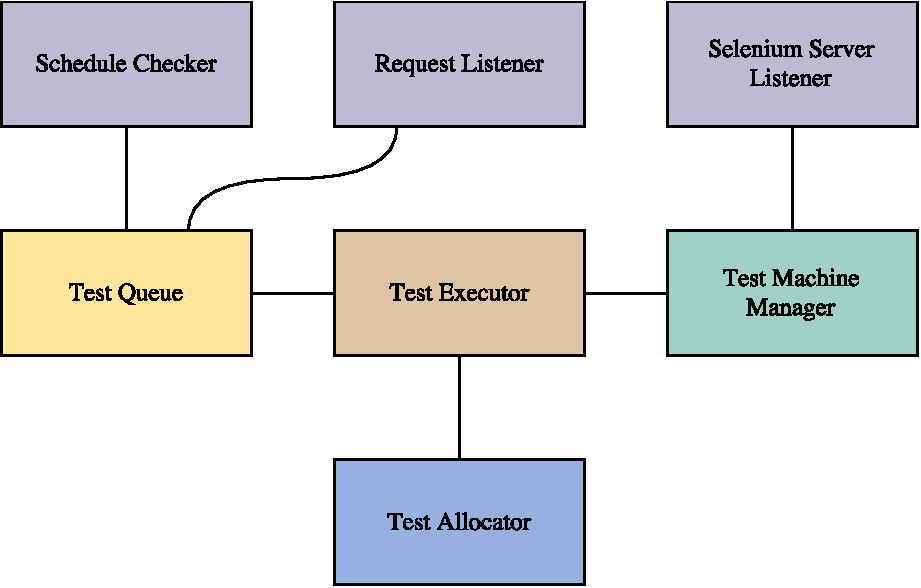
\includegraphics[width=\textwidth]{figures/new/controller3.pdf}
    \thisfloatpagestyle{plain}
    \caption{Controller Structure}
    \label{fig.controller_structure}
\end{figure}


\noindent The \emph{controller} consists of multiple processes running in different threads. Figure \ref{fig.controller_structure} shows the inner structure. Each of the modules in the figure will be explained in this Section.

\subsubsection{Selenium Server Listener}
After starting the Selenium Grid Hub as described in Section\ref{section.selenium} using configuration details found in the configuration file, the main job of the Selenium Server Listener is to listen to the output from the Selenium Standalone Server. This means that when a node connects or disconnects to the system, the Selenium Server Listener is notified. When one of these events happens, it sends notice to its instance of the Test Machine Manager.

\subsubsection{Test Machine Manager}

\improvement[inline]{TODO (Might re-implement this, so will wait with writing this subsection.)}

\subsubsection{Request Listener}

All test executions managed by \toolname \space are either requested for immediate execution or scheduled ahead of time. There are two different modules in the controller each handling one of these.

The \emph{Request Listener} constantly listens to a port specified in the configuration file. When a user triggers the \emph{Execute Now} action from the dashboard, all necessary information about the tests being requested for execution is packed as a \emph{JSON} string and sent to the controller using a TCP/IP protocol in Python's \emph{socket} library.

Upon receiving a request, the request listener unpacks the JSON string and creates a list of corresponding \emph{test} objects. The list is then forwarded to the \emph{queue}.


\subsubsection{Schedule Listener}
\improvement[inline]{TODO}
\comment{\info{Might re-implement this part to improve efficiency.}}











\subsubsection{Queue}

As test executions are requested by the controller, each individual test case is placed in an execution queue. The queuing system is made up of four distinct queues with corresponding descending priorities; one for urgent execution, one for immediate execution, one for planned execution, and one for trial execution. Each test case is placed in a queue according to which action triggered their request to be executed. If the request was identified by the request listener, it is placed in the queue for immediate executions. If it was the schedule listener that identified it, the test is placed in the queue for planned executions. If the test case have just been uploaded or updated, it will be placed in the queue for trial execution. The urgent queue is where test cases that were not executed because the test node they were allocated to crashed.

Sometimes a planned execution and an immediate execution of the same test case with the same browser and platform specifications can be requested at the same time. A similar situation could occur when two schedule objects that are due at the same time includes the same test case with the same specifications. Scenarios such as these could potentially lead to time and resources wasted by performing the same job twice. To avoid incidents in which two identical test cases are executed at the same time, a duplicate check is performed each time a test case is added to one of the queues. If there are duplicates, the test case is removed from the queue with the lowest priority.

The test case executor always checks the immediate queue first, then the planned queue, and lastly the trial queue. If the test executor finds test cases in any of the queues, it empties the queue and handles the containing test cases as a group.

\subsubsection{Test Execution}

After test cases have been retrieved from the queue, allocated amongst the pool of available test machines (Section \ref{allocation}), and sorted, it is time for execution.

A thread is started for each of the test machines. In these threads, each test case is started as a subprocess using a shell command in which information regarding the desired test node and browser of the test execution are passed to the test script as arguments.

Immediately before a test case is executed, the test node is pinged to see if the connection is still up. This check is also done immediately after any failed test. If the node has crashed or otherwise failed before or during the execution, the test cases are moved to the queue for urgent executions, and attempted executed once the current test run has finished.

If there none of the test machines match the required browser/platform specification of a given test case, the test will not be executed; it will appear in the execution log, but will be marked as \betterfakesc{Not Executed}.




%%%%%%%%%%%%%%%%%%%%%%%%%%%%%%%%
% SUBSECTION: Allocation Machanism
%%%%%%%%%%%%%%%%%%%%%%%%%%%%%%%%
\subsection{Allocation Mechanism}\label{allocation}

Since the test type intended for \toolname \space generally runs slowly, designing a mechanism that would efficiently allocate tests to test machines in an attempt to minimize the duration it takes to find and execute the schedule. This mechanism has been named \emph{Opti-X}, and will be thoroughly described in the following subsection. As explained in Chapter \ref{chapter.background}, an alternative allocation mechanism has also been implemented using Google's OR-Tools library, and has been used in the evaluation process of Opti-X, which will be presented in the next chapter. The alternative allocation mechanism has been named \emph{OR-X}, and implementation details will be explained subsequently.

\subsubsection{Opti-X}

The Opti-X allocation mechanism consists of a sequence three steps; sorting, initial allocation and enhancement iterations. It can be seen as an extended greedy algorithm, and will be explained in this section.

In order to give a better understanding of how the algorithm works, a demonstration example will be used throughout the explanation. In this example, we assume that there are three test machines connected to the system, as well as the test suite listed in table \ref{testsuite}. Note that the durations of the tests intended for \toolname \space generally range from 30 to 90 seconds, and this example deliberately uses shorter durations to better illustrate the mechanism.

\begin{table}[h!]
  \begin{tabular}{c c c}
    \hline
    \textbf{Test} & \textbf{Duration} & \textbf{Executable on}\\
    \hline
    $t_{1}$     &   6   &   $m_{1}$, $m_{2}$, $m_{3}$\\
    $t_{2}$     &   3   &   $m_{1}$, $m_{2}$, $m_{3}$\\
    $t_{3}$     &   8   &   $m_{1}$, $m_{2}$, $m_{3}$\\
    $t_{4}$     &   5   &   $m_{1}$, $m_{2}$, $m_{3}$\\
    $t_{5}$     &   3   &   $m_{1}$, $m_{2}$, $m_{3}$\\
    $t_{6}$     &   4   &   $m_{1}$, $m_{2}$, $m_{3}$\\
    $t_{7}$     &   7   &   $m_{1}$\\
    $t_{8}$     &   3   &   $m_{2}$\\
    $t_{9}$     &   9   &   $m_{3}$\\
    $t_{10}$    &   5   &   $m_{1}$, $m_{3}$\\
    \hline
  \end{tabular}
  \centering
  \caption{Example Test Suite}
  \label{testsuite}
\end{table}

\comment{(extended) greedy algorithm with iterations.}

%\vspace{7px}
\noindent \textbf{\betterfakesc{Sorting}}\\
\noindent The first step is a preparation for the initial allocation. The sorting does not play a crucial role in the allocation mechanism, but is creates an excellent starting point as the tests are sorted in a way that makes them well suited for the initial allocation in the next step. If toward the end of the allocation process there would only be left tests that could run on a certain machine, the overall execution time could be greatly affected, so the sorting avoids this by ordering them fittingly beforehand.

The test set is first divided into subsets depending on the number of machines they can be executed on. Each of the subsets is then sorted by their estimated duration in descending order, so that the longest tests are placed first and the shortest are placed last. The list is then assembled again.

\begin{figure}[ptb]
    \centering
    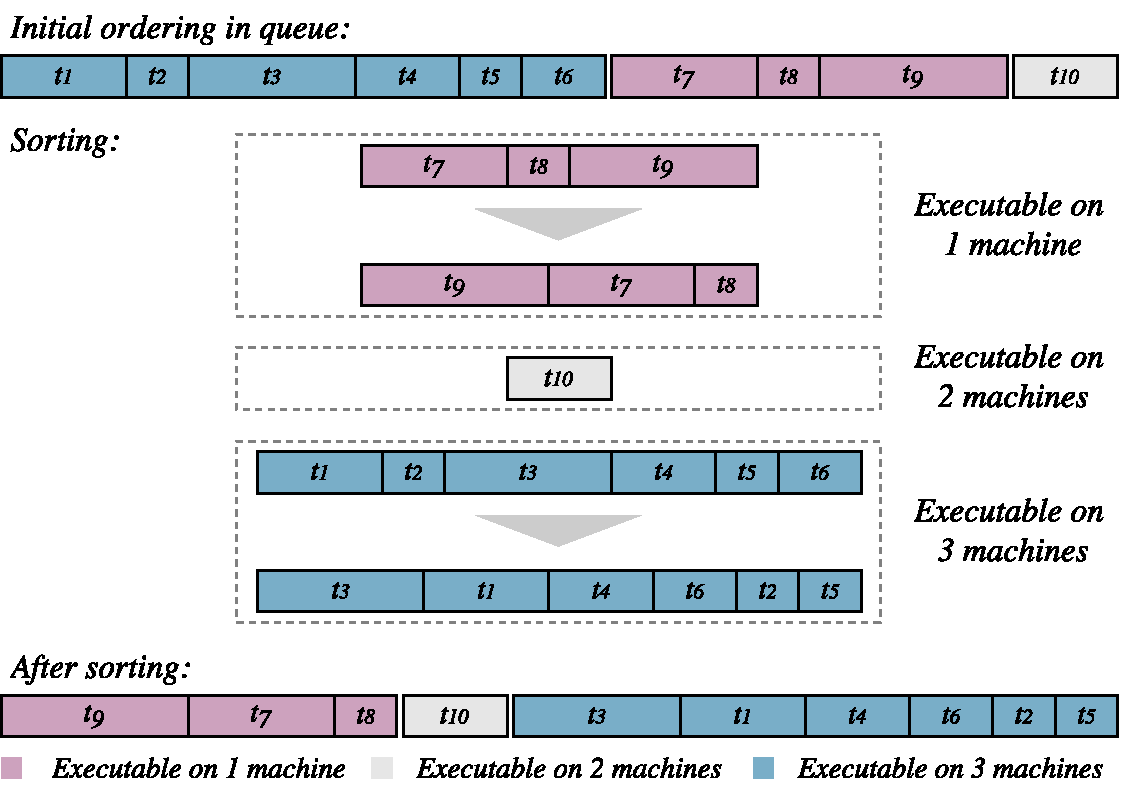
\includegraphics[width=\textwidth]{figures/new/sorting.pdf}
    \thisfloatpagestyle{plain}
    \caption{Sorting of Example Test Suite}
    \label{fig.sorted_test_suite}
\end{figure}

Figure \ref{fig.sorted_test_suite} illustrates how the sorting method works with the example test suite introduced earlier. Since $t_{7}$, $t_{8}$ and $t_{9}$ can only be executed on a single machine each, these are placed first in descending order of their duration. $t_{10}$, which can be executed on two machines comes after. Finally, tests $t_{1}$ through $t_{6}$, which can run on all of the machines, are ordered and added to the test list.






\vspace{7px}
\noindent \textbf{\betterfakesc{Initial Allocation}}\\
\noindent The initial allocation is a greedy algorithm, which means that it always makes a locally optimal choice in the hopes that it will give the best result in the end \cite{Algorithms}. Greedy algorithms are powerful and work well for an extensive spectrum of problems. Creating a greedy algorithm was a suitable choice for this problem.

This step creates the foundation of the test allocations. After being sorted, the test list is looped through, and the tests are allocated one by one, starting with the \emph{longest} of the tests that are executable on the \emph{fewest} machines. Each test is initially allocated to the machine that currently has the shortest overall duration among the machines that the test is executable on.

\begin{figure}[h]
    \centering
    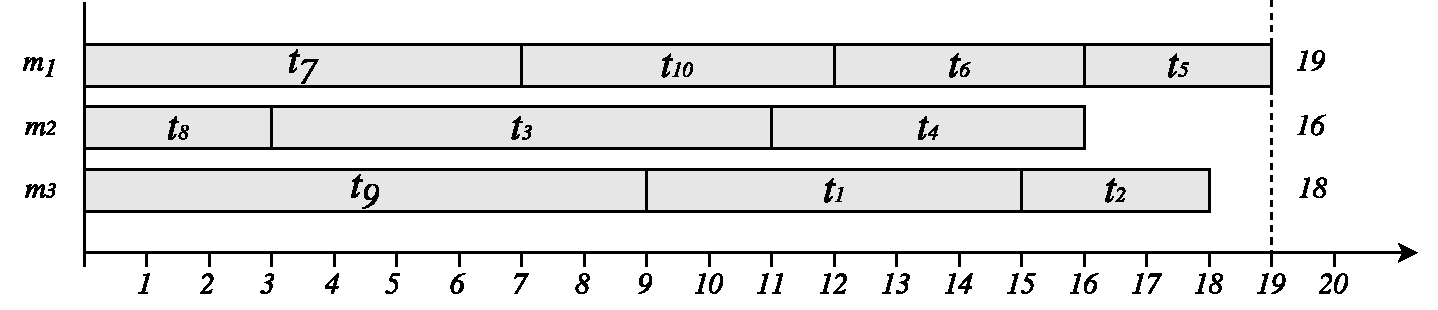
\includegraphics[width=\textwidth]{figures/new/initial_allocation2.pdf}
    %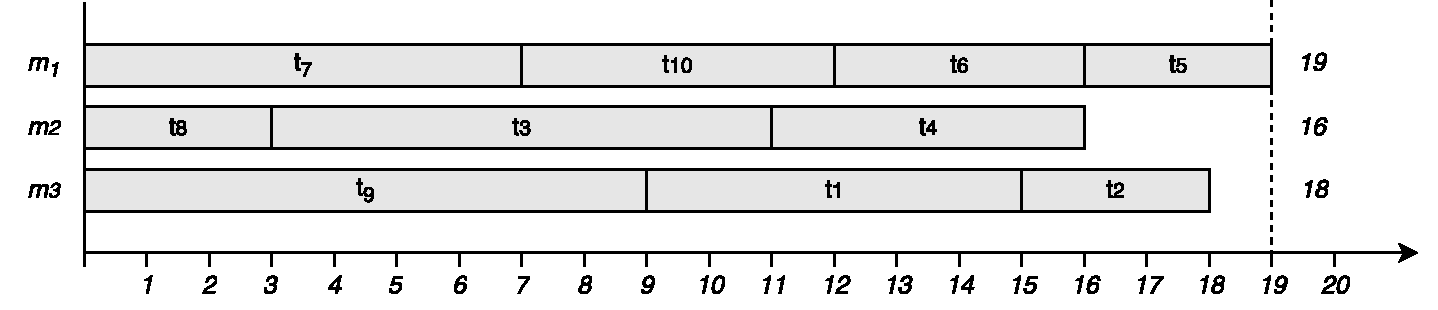
\includegraphics[width=\textwidth]{figures/initial_allocation.pdf}
    \caption{Initial Allocation of Example Test Suite}
    \label{fig.initial_allocation}
\end{figure}

Figure \ref{fig.initial_allocation} shows how the test suite is initially allocated among the test machines. $t_{9}$, $t_{7}$ and $t_{8}$ are first allocated to $m_{3}$, $m_{1}$ and $m_{2}$ one by one, as each of them can only be executed on that machine. $t_{10}$ can be executed on both $m_{3}$ and $m_{1}$, but as the latter currently has the shortest overall execution time, this is the machine it is allocated to. The remaining tests are allocated in the same way. After the initial allocation is finished, the overall execution time is 19. However, the total durations among the machines are slightly uneven, so there might be room for improvement. This will be examined in the last step of Opti-X.






\vspace{7px}
\noindent \textbf{\betterfakesc{Enhancement Iterations}}\\
\noindent Greedy algorithms are simple, yet efficient, and provide adequate results most of the time. However, they do not always yield optimal solutions. In order to improve the result, an additional step has been included in the Opti-X. This is the most complex element in the process.

The basic idea behind the iteration step is to find subsets of tests among two machines and swap the two subsets that will decrease the total duration of the two machines the most. The subject of each iteration is the machine that currently has the longest execution time. In the case of the example test suite, this is $m_{1}$. This will be referred to as the \emph{swapper}. Each of the remaining machines are addressed one by one, starting with $m_{2}$, which is a \emph{swappee} candidate. The tests that are currently allocated to the swapper, but also executable on the swappee candidate are retrieved, which in this case is $t_{5}$ and $t_{6}$. A list of all possible subsets from this set is then created. This is done by using Python's \emph{itertools} library. The same is done the other way around, with $t_{3}$ and $t_{4}$ for the swappee candidate. After this, we examine how each swap would affect the overall total duration of the two machines in question. After comparing all subsets, it is concluded that the best swap is $t_{5}$ and $t_{6}$ from $m_{1}$ for $t_{4}$ from $m_{2}$, which will decrease the overall duration among the two machines with 1 time unit. Since $m_{3}$ can not provide any better options, this swap is conducted. This process will repeat until there is no way to improve the allocations, which in this case is after one swap. In this example, \toolname \space found an optimal solution to the optimization problem. Figure \ref{fig.iteration} shows how the subset swap is conducted, and how it affects the overall duration.

Upon evaluating each swappee candidate, a naive best-case duration is calculated by adding the durations of all the tests from the two machines and dividing the sum by two. If the time used to search for the best swap exceeds the difference between the total duration of the swapper (here: 19), and this best scenario duration (here: $\frac{19+17}{2} = 18$), which in this case is $1$, we will continue to the next swappee candidate. This means that we will examine the subsets of $m_{2}$ for maximum 1 unit of time.

%In an attempt to save time, the subsets are sorted according to their total durations; the swapper subsets descending and the swappee subsets ascending. This ensures that the subsets with the longest total durations are attempted removed from the swapper first.

\begin{figure}[t]
    \centering
    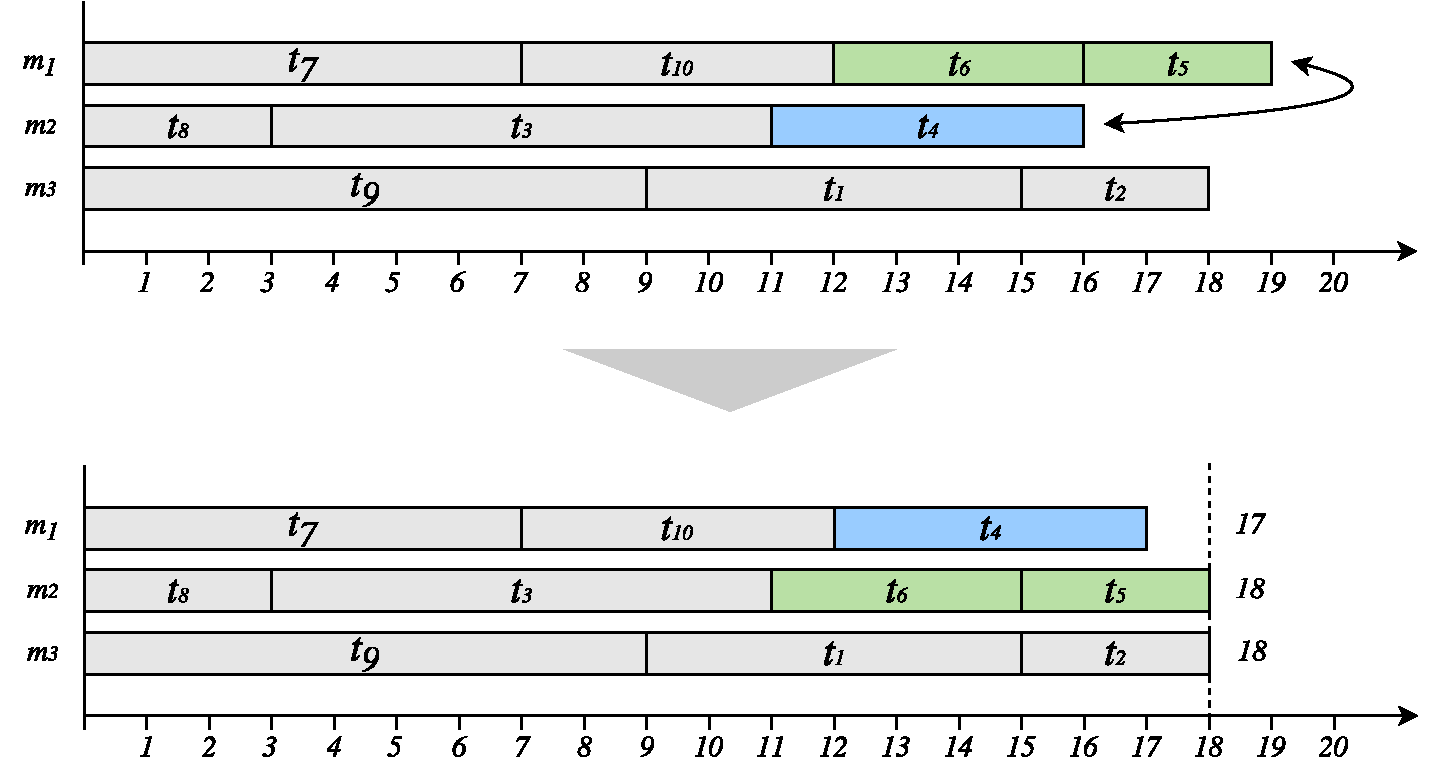
\includegraphics[width=\textwidth]{figures/new/iteration2.pdf}
    %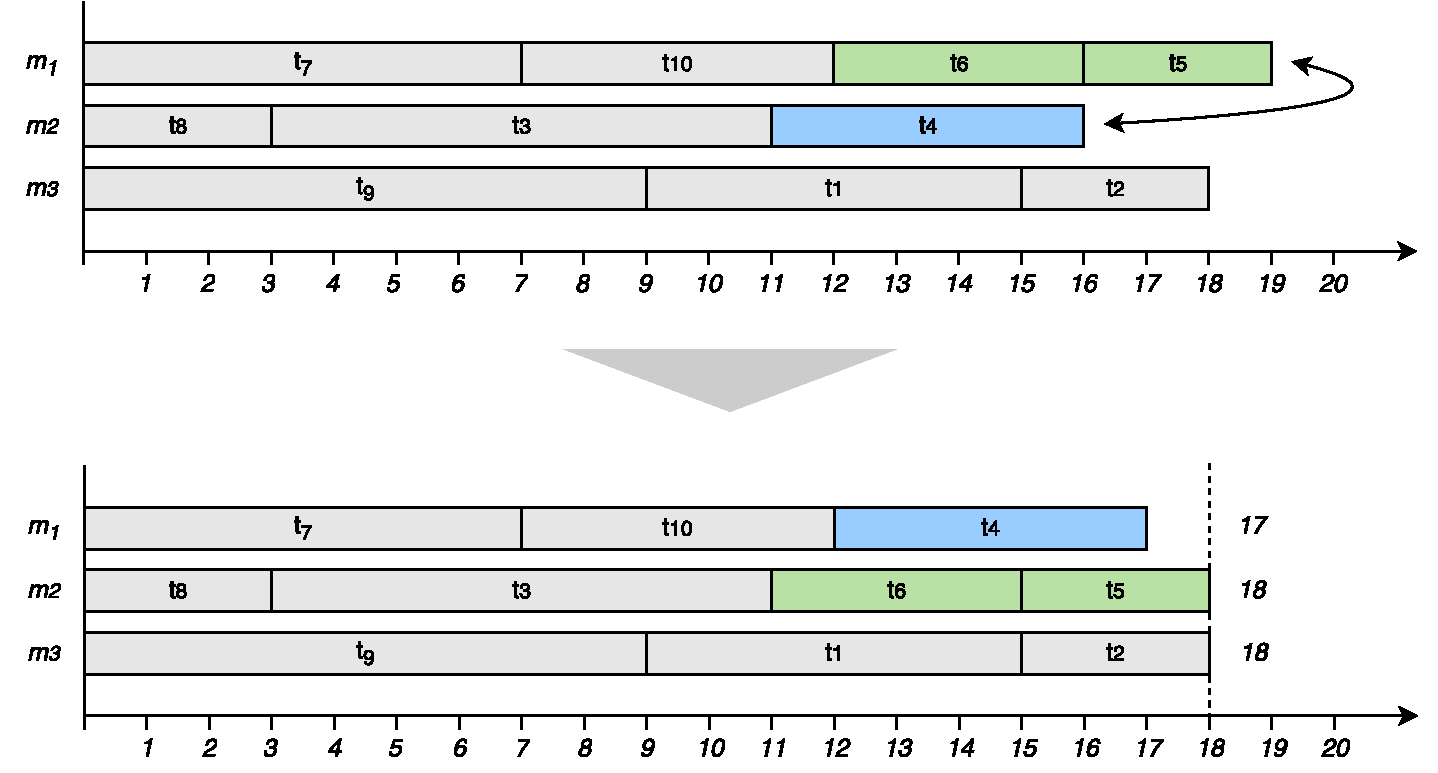
\includegraphics[width=\textwidth]{figures/iterations2.pdf}
    \caption{Enhancement Iteration of Example Test Suite}
    \label{fig.iteration}
\end{figure}

Sometimes, however, we want to stop the searching earlier, as continuing is no longer beneficial. For that reason, two stop criteria are introduced:

\begin{enumerate}
    \item When the iteration method is first called, a naive best-case overall duration value is calculated by dividing the sum of all test durations by the number of machines available. Once the time difference between this value and the maximum machine duration is exceeded, the iteration process will stop.
    \item There is a timeout set to 60 seconds. If the iterations still are not finished at this point, the method will be terminated, and the allocations arrived at that point will be kept.
\end{enumerate}

During the development phase, a clear problem stood out; creation of subset lists from extremely large interchangeable test sets between two machines could take several minutes, and sometimes even lead to memory leaks so that the whole system crashed. This was because there was simply too many possible subsets. To work around this problem, a restriction of the maximum size of the subsets had to be established. Through trial and error, the following was decided upon:

\[
\hfill
    f(x)=\left\{
        \begin{array}{l l}
          x         &   \hspace{20px} if \hspace{32px} x < 10\\
          20-x      &   \hspace{20px} if \ 10 \leq x < 20 \\
          1         &   \hspace{20px} if \ 20 \leq x
        \end{array}
    \right.
\hfill
\]

Thus, if the number of interchangeable tests are 19 or more, the subset list will only consist or singular tests in addition to the empty set. Although not optimal, this was a compromise that helped on the problem. This means that for large interchangeable sets, tests can only be swapped one against one or moved from one machine to another. It is therefore sensible to think that better swaps might exist, although identifying these would take too much time and potentially lead to memory leaks.  Figure \ref{fig.subsets} shows a plot of $f(x)$.

\begin{figure}[h]
    \centering
    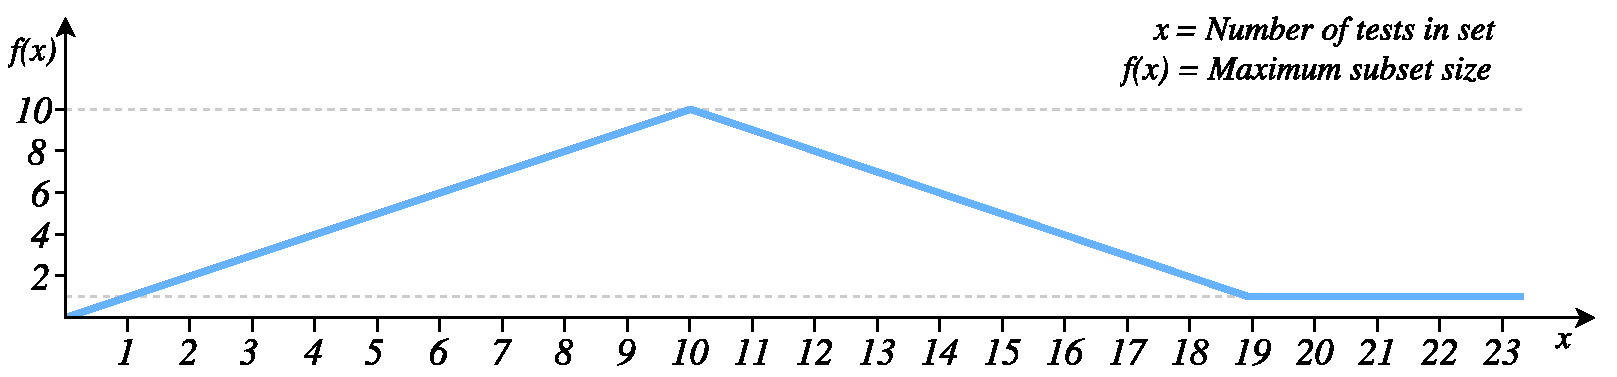
\includegraphics[width=\textwidth]{figures/new/subset_sizes.pdf}
    %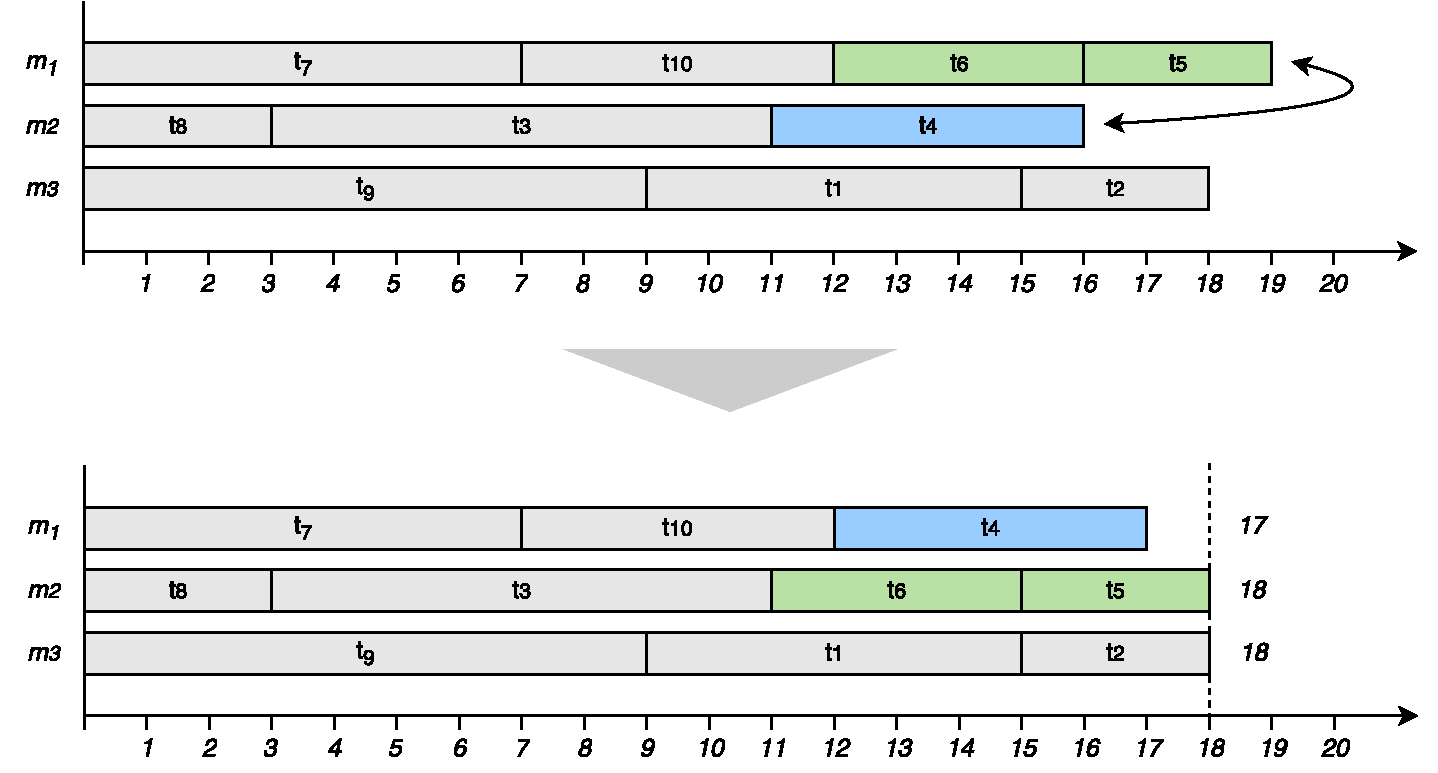
\includegraphics[width=\textwidth]{figures/iterations2.pdf}
    \caption{Maximum Subset Sizes}
    \label{fig.subsets}
\end{figure}

Because of the stop criteria described earlier and the subset size restriction, \toolname \space cannot \emph{guarantee} to find an optimal solution to the allocation problem. However, as explained in Section \ref{subsection.cp}, the objective of the optimization problem is to minimize the total time, which means that the time used to search for the best solution is also of high importance, and should be prioritized as such.

\subsubsection{OR-X}

The implementation of OR-X is of the same style as the OR-Tools example shown in \lstlistingname \space \ref{listing.or_tools} in Chapter \ref{chapter.technology}, but more complex. OR-X takes two lists; one containing the durations of the tests, and another containing which machines each test is executable on. OR-Tools does not support decimal values, so all values in the durations list must be converted to integer values. The \emph{executable on} list is nested, with one list belonging to each test. These inner lists contain binary values representing whether or not the test can be executed on a given machine. It is then added as a constraint that each test should be allocated to exactly one machine, and as the objective that the overall duration should be minimized.

However, there was one major issue upon the implementation of OR-X. It was not possible to interrupt or time out the \emph{NextSolution} method. For very small data sets, this was not a problem, but once the data sets grew slightly bigger and the combination possibilities grew rapidly, the method could take hours. This meant that a set of stop criteria had to be introduced. However, the problem could still not be solved by running the solver in a separate thread, as there is no integrated method of terminating regular threads in Python to the best of the authors knowledge. the problem was solved by introducing Python's \emph{multiprocessing} library.

The solving method is started as a \emph{Process} from the multiprocessing library. In order to allow two processes to share lists, a \emph{Manager} is needed, and to ensure synchronization, a \emph{Lock} has been used. \lstlistingname \space \ref{listing.orx_multiprocess} shows how these multiprocessing modules are used in OR-X.

\vspace{4mm}
\begin{lstlisting}[caption=OR-X Multiprocessing, label={listing.orx_multiprocess}]
from multiprocessing import Process, Manager, Lock

manager       = Manager()
allocations   = manager.dict()
max_durations = manager.list()
last_updated  = manager.list()
lock          = Lock()

// ...

p = Process(target=find_solution, args=(durations, executable_on, allocations, max_durations, last_updated, lock))
p.start()

while p.is_alive():
  if lock.acquire():
    if <stop criteria fulfilled>:
      p.terminate()
      break
    lock.release()

// ...

def solution_loop(self, durations, executable_on, shared_allocations, max_durations, last_updated, lock):
    // ...
    
    while solver.NextSolution():
      lock.acquire()
      // ...
      lock.release()
\end{lstlisting}

\noindent OR-X will be terminated if one of the following stop criteria are fulfilled:

\begin{itemize}
    \item The search for an enhancement has taken 100 times as long as it took to find the previous enhancement.
    \item The previous enhancement took 10 times as long to find than the enhancement itself.
    \item 60 seconds have passed (timeout).
\end{itemize}







%%%%%%%%%%%%%%%%%%%%%%%%%%%%%%%%
% SUBSECTION: Database
%%%%%%%%%%%%%%%%%%%%%%%%%%%%%%%%
\subsection{Database}

The relational database management system (RDBMS) SQLite can be regarded as a light-weight substitute to other SQL based database engines. Benefits to SQLite compared to these other database systems include its being self-contained and serverless, and the database is contained in a single disk file \cite{https://www.sqlite.org/about.html}. For convenience concerning submission, SQLite was the preferred choice for this project. However, another SQL database engine can replace it with little effort if needed.

As explained in Chapter \ref{chapter.technology}, Django data models define the database layout, and each model typically maps to an individual table in the database. SQL code for creating the database itself and the tables within it are all auto-generated by Django, based on the implementations of the models. If a m-to-n relation between two different models are defined in the model implementations, a separate relationship table is created in the database to cover this. The auto-generated SQL files covering creations and changes to the tables related to test automation are all placed under \emph{testautomation} $\rightarrow$ \emph{migrations} by default. When a change has been done to one of the models, a new migration can be created by performing a few shell commands \cite{https://docs.djangoproject.com/en/1.9/topics/migrations/}.

The database can be accessed either by writing raw SQL queries, or through Django's API for database abstraction. The former approach was first implemented in this system, but was then changed to the latter, as it was cleaner and more consistent with the implementation of the rest of the project. It was also interesting to use a different practice of database communications than the more commonly used raw SQL queries. \lstlistingname \space \ref{listing.db} shows a simplified example of how an \betterfakesc{insert} statement is conducted using this approach. In this example, the implementation of the \betterfakesc{Log} model is imported, and then an object of this type is created with pseudo values for a small set of attributes. Line 5 in the listing represents the transaction execution and commit. Note that implementation of such object creations includes several more attributes than what is shown in this example.

\vspace{4mm}
\begin{lstlisting}[caption=Database Communication Using Abstraction API, label={listing.db}]
from testautomation.models import Log
from datetime import datetime
 
l = Log(title='test1', result=1, execution_time=datetime.utcnow())
l.save()
\end{lstlisting}

\noindent In addition to providing excellent readability, the abstraction greatly decreases the required number of code lines needed to achieve the same result compared to executing raw SQL queries. This is because the database location does not need to be stated, connection with the database does not need to be programmatically established and then closed when the transaction is finished, and so forth. The abstraction takes care of all of this. The running time of the two approaches also proved to be approximately the same after testing both methods. Other types of queries such as \betterfakesc{Select}, \betterfakesc{Update} and \betterfakesc{Delete} are also supported with this API.

Information about test cases, test groups, schedules, logs as well as user information is all stored in various tables of the database. Figure \ref{fig.db_er} shows the Entity-Relationship (ER) diagram of the database.


\begin{figure}[p]
    \centering
    \thisfloatpagestyle{empty}
    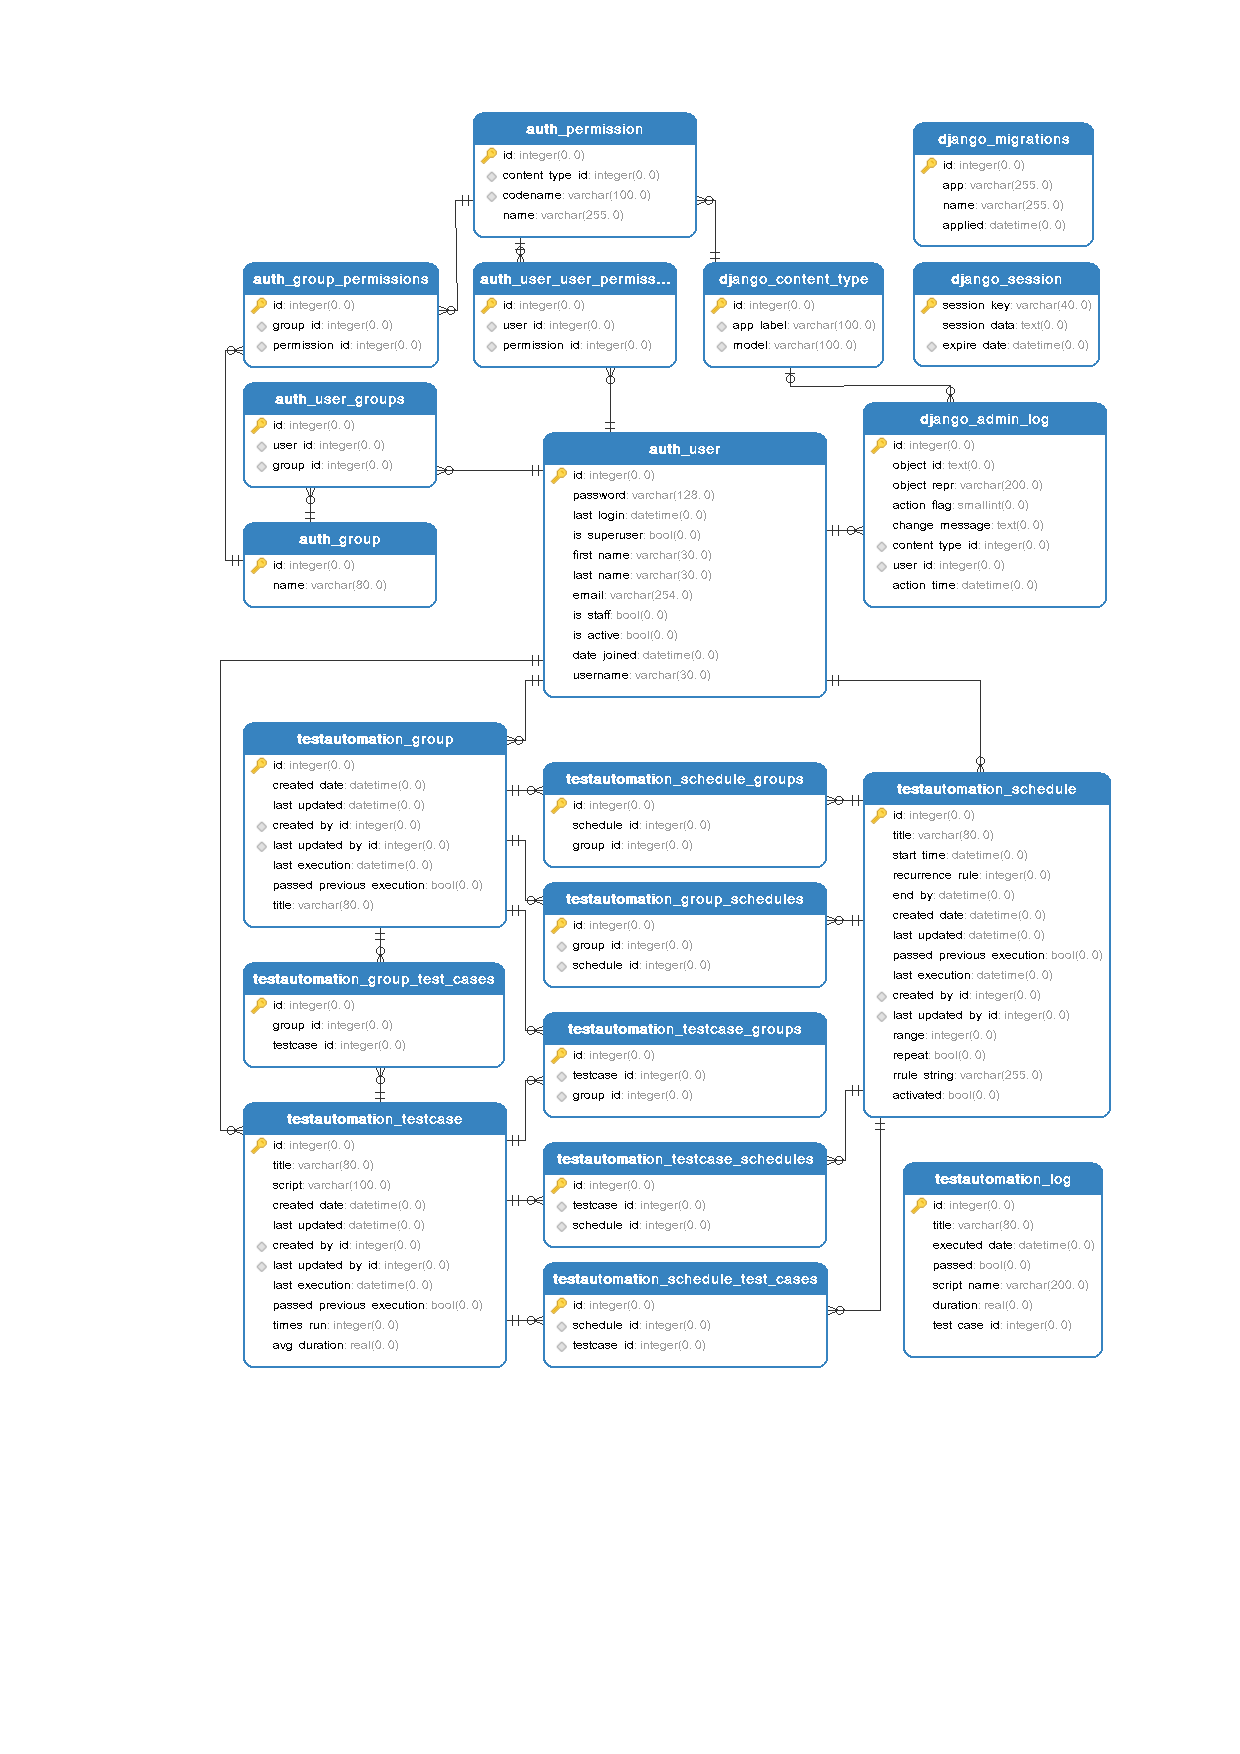
\includegraphics[width=\textwidth,height=\textheight]{figures/er_diagram.pdf}
    \caption{ER Diagram of Database}
    \label{fig.db_er}
\end{figure}

All timestamps stored in the database are in the Coordinated Universal Time (UTC) standard, which, as the name suggests, is universal, and therefore independent of time zones. The time zone used in the web service is set to 'Europe/Oslo' in the Django settings file. Whenever a timestamp is shown on screen, it is first converted to the specified time zone using Django's \emph{timezone} library. If the user is located in a different time zone than the one specified in the settings, a label explaining that the computer is \emph{xx} hours ahead or behind of server time is displayed next to any \emph{datetime} picker, such as in the schedule creation form.

\noindent Storing timestamps according to the UTC standard rather than the current time zone can be considered good practice for multiple reasons. Firstly, there can be no ambiguity. Confusion and misunderstandings related to conversion across different time zones will be avoided, which also means that timestamp calculations are simple. Further, there can be no invalid dates linked to daylight savings time. Moreover, if the server were to be moved to a different time zone, timestamps would have to be converted.





%%%%%%%%%%%%%%%%%%%%%%%%%%%%%%%%
% SUBSECTION: Dashboard
%%%%%%%%%%%%%%%%%%%%%%%%%%%%%%%%
\subsection{Dashboard}

\improvement[inline]{TODO: Write section intro}
\comment{\todo[inline]{TODO: Describe maybe a little bit more how django/django admin works? Some parts are automatic and some are implemented. Some stuff are overrided, some stuff are extended, etc}}

\subsubsection{Models}

With Django, data models provides the foundations on which database tables are created and maintained. A model implementation can be seen as a Python equivalent to an SQL \betterfakesc{Create Table} statement. Model implementations are translated to SQL and executed by Django. Each model, which is a subclass of \emph{django.db.models.Model}, represents a table in the database, and each model field represents a database field. Similar to SQL, the data type of each field along with any other specifications such as the maximum length of a text field, default values and help text can be passed as \emph{field option} parameters.

The models are located in \emph{testautomation} $\rightarrow$ \emph{models.py}. In this file, model specifications of test cases, groups, schedules and logs are implemented.

Additionally, models can contain elements that are not linked to the database, such as a field of which a value is based on a function that is performed each time the value is requested displayed. These functions can return primitive data types, but they can also contain HTML tags, so the content can be customized. Such functions are used in several of the models. For instance in the test case module, there are one function that query the \betterfakesc{Log} table in the database, and counts number of instances linked to the particular test case. Average duration and previous execution date are retrieved in a similar manner.

\vspace{4mm}
\begin{lstlisting}[caption=Model Implementation, label={listing.model}]
from django.db import models
 
class TestCase(models.Model):
    title = models.CharField(max_length=80)
    script = models.FileField(upload_to='scripts')
    
    def times_run(self):
        tr = # perform query
        return tr
\end{lstlisting}

\noindent \lstlistingname \space \ref{listing.model} shows a reduced adaption of how the test case model has been implemented. This model contains two model fields and a function. The \emph{script} field is of the type \emph{model.FileField}, and the directory that the files should be uploaded to is passed as a parameter. The file upload itself is taken care of by Django.





\subsubsection{Admin}

\improvement[inline]{TODO: Write introduction to this subsection}

\vspace{4mm}
\begin{lstlisting}[caption=Implementation of Model in Administrator Interface, label={listing.modeladmin}]
from django.contrib import admin
from .models import TestCase

class TestCaseAdmin(admin.ModelAdmin):
    list_display = ('title', 'times_run', 'avg_dur')
    search_fields = ['title',]
    fields = ('title', 'script')
 
admin.site.register(TestCase, TestCaseAdmin)
\end{lstlisting}

\noindent \lstlistingname \space \ref{listing.modeladmin} shows a very reduced interpretation of how the test case model is represented in the administrator interface. This adaption builds on the model implementation from \lstlistingname \space \ref{listing.model}. Model administrator representations are subclasses of \emph{django.contrib.admin.ModelAdmin}, and specifies how the model should be represented in the administrator interface. This interpretation specifies values of three of the many ModelAdmin options; which fields of the model should be displayed in the overview list of the test case module ('list\_display'), which fields should be searchable ('search\_fields') and which which fields should be present in the creation/change form ('fields'). Line 9 registers the model to the administrator interface with the specifications stated in the TestCaseAdmin class.

In the actual implementations of the model admin representations, a number of additional fields and specifications are also included. Custom forms with particular validation functionality can be integrated with the creation/change form. This has been done with test case objects to ensure that only test scripts that fulfill certain criteria can be uploaded. Admin actions are also implemented here.

\improvement{TODO: List and describe the implemented admin actions?}

\subsubsection{Issue Tracker Reporting}
\improvement[inline]{TODO}
\comment{TODO - JIRA Rest API, etc.}

\subsubsection{Management of Test Machines}
\improvement[inline]{TODO}

\subsubsection{Event Recurrence}
\betterfakesc{Rrule}, short for \emph{recurrence rule}, is a part of to a Python library called \emph{dateutil}, which provides an extension to Python's \betterfakesc{datetime} module. It  is a small and fast library used in \toolname \space to specify recurrence patterns of test executions. \betterfakesc{Rrule} instances can be implemented multiple ways. In this project, it is achieved through passing a string with a specific format, containing information about the desired recurrence constraints. This string is stored in the database, and can be used at any point to create an \betterfakesc{rrule} instance in order to inquire when the next event should take place. An example of such a string, how \betterfakesc{rrule} instances are created in this project, and how the next occurrence is retrieved, can be seen in \lstlistingname \space \ref{listing.rrule}.

\vspace{4mm}
\begin{lstlisting}[caption=Recursion Rule, label={listing.rrule}]
from dateutil.rrule import rrulestr
from datetime import datetime

rule_string = "DTSTART:20160615T160000\nRRULE:FREQ=WEEKLY"
rule = rrulestr(rule_string)
 
print rule.after(datetime.now())
 
>>> 2016-06-15 16:00:00
\end{lstlisting}

\noindent The string in the listing above is used to create an rrule instance in which the first occurrence is set to the 15\textsuperscript{th} of June 2016 at 4 pm, and repeats weekly. In addition to the recurrence properties shown in the listing above, the library provides an extensive number of recurrence options, including end date, occurrence count and interval.

\comment{
    \missingfigure[figwidth=\textwidth]{Screenshot of filled-in schedule form? With corresponding rrulestr?}
    
    The recurrence rule strings in this project are built dynamically when a schedule object is created or updated. If the schedule creation form shown in Figure \ref{fig.rrule} is submitted, it would produce the following 
}

The recurrence rule strings in this project are built dynamically when a schedule object is created or edited. In the test case, group and schedule modules of \toolname, recurrence rule strings are used to create \betterfakesc{rrule} instances, which again are used to find out the time of the next planned execution for the particular test case, group or schedule. \betterfakesc{Rrule} instances are also created by the controller to check when the next test run is scheduled.


\comment{
\subsection{Other?}
\change[inline]{
Include data flow - what happens from someone clicks "Execute now" and until the result is shown in the log? (FLOW CHARTS!)
How are Jira issues created?

Include a (detailed?) figure system architecture of how the system is integrated. Start by explaining how the different parts talk to each other. In the beginning, consider the controller as a unit, give more detailed descriptions of objects, listeners, algorithms, etc later.

How does the scheduling algorithm work? Try to be as academic as possible - use academic language when describing the algorithm; define the problem mathematically, use graphs and flow charts, use an example.

Two types of scheduling:
- Optimal allocation and scheduling of test cases in a test run
- Planned scheduling of future test run with recurrence option (rrule, rrulestr)
}

\comment{SELENIUM GRID is load balanced, but otherwise chooses which machine to execute a test on sporadically. There is no documented way of specifying which node to execute a specific test on, but it can be done by adding some unique information to each node upon setup, and to use the same piece of information in the capability section in the setup function of the test script. https://groups.google.com/forum/#!topic/selenium-users/PRsEBcbpNlM}

\todo[inline]{
Scheduling algorithm:

job-machine-matrix / test case-node matrix (binary) (shows which machine can run each test case, which machines each test case can run on)}

    [
        \hfill
        \mathbb{M} = \kbordermatrix{
                  & tc_{1} & tc_{2} & tc_{3} &        & tc_{n} \\
            m_{1} & x_{11} & x_{12} & x_{13} & \dots  & x_{1n} \\
            m_{2} & x_{21} & x_{22} & x_{23} & \dots  & x_{2n} \\
                  & \vdots & \vdots & \vdots & \ddots & \vdots \\
            m_{d} & x_{d1} & x_{d2} & x_{d3} & \dots  & x_{dn}
        }
        \hfill
    ]



http://stackoverflow.com/questions/5674253/a-task-job-scheduling-problem

\comment{
\info[inline]{
Constraints:
- Each test case must be executed once and once only
- Machines can execute test cases in paralell
- Execution time is assumed to be machine independent
- Each machine can only execute one test case at a time
- Heterogeneous environment (at least not necessarily homogeneous) - different OS and OS versions, different browsers and browser versions - not all test cases can be executed on each machine

Objective: Minimizing running time


From TC-Sched:
time-constrained cumulative scheduling constraint-based technique because 1) it allows
us to keep fine-grained control on the time allocated to the
constraint solving process (i.e., time-constrained), 2) it encodes
exclusive resource use with constraints (i.e., constraint-based),
and 3) it solves the problem by using the CUMULATIVES constraint.
The TC-Sched method is composed of three elements,
namely, the constraint model described in Section III-A, the
search procedure described in Section III-B, and the timeconstrained
minimization process described in Section III-C.


Constraints:
-Non-cumulative scheduling: Two test cases cannot be executed at the same time on a single machine.
-Non-preemptive scheduling: The execution of a test case cannot be temporarily interrupted for the running machine to execute another test case instead.
-Non-shared resources: When a test case uses a global resource, no other test case using the same resource can be executed at the same time.
-Machine-independent execution time: The execution time of a test case is assumed to be independent of the machine on which it is run. This is a reasonable assumption for test cases in which the time is dominated by external physical factors such as a robot’s motion, the opening of a valve, or sending an Ethernet frame. Such test cases typically have execution times that are uncorrelated with machine performance (e.g., CPU type, CPU frequency, operating system). In any case, a sufficient over-approximation of the execution time will satisfy the assumption.


EXPERIMENTAL EVALUATION

This section presents our findings from experimentally evaluating TC-Sched. To this end, we address the three following
research questions:

RQ1: How does the solution provided by TC-Sched compare with simpler scheduling methods in terms of the time needed to execute the schedule? RQ1 states the crucial question of wether using strong constraint optimisation tools is useful or
not in a context where cheaper-to-run methods are available at almost no cost of implementation.
RQ2: For TC-Sched, will an increased investment in the solving time reduce the overall time of a CI cycle? This question
is about finding the most appropriate trade-off between the solving time and the execution time of the test schedule.
RQ3: Can TC-Sched effectively handle industrial cases which contain up to hundreds of test cases and tens of machines?}
}
}
\section{Evaluation}\label{chapter.discussion}
\thispagestyle{plain}

This chapter opens with introducing a collection of test sets used to measure the performance of the allocations mechanism OptiX through experiments, and compare it to the performance of ORX on the same collection. The results are evaluated and discussed, followed by an assessment of factors that may threat the validity of the results obtained in the experimental phase. \toolname \space is then discussed and evaluated as a whole, before the chapter rounds off by discussing the return on the investment put into this project.

\comment{
\subsection{Research Questions?}
Look at Mortens report for inspiration. Or maybe not?
}

\subsection{Experimental Evaluation of Test Allocation}
%\improvement[inline]{TODO}
\comment{- Present test data, run experimental tests and create tables and charts, include a second version of ORX that runs without interruption in order to compare OptiX and ORX to the actual optimal overall running duration!}

In order to measure and evaluate the performance of OptiX, which represented a major objective in this project, an experimental evaluation was performed on OptiX as well as on ORX to establish benchmark values.

The test data used in the experimental evaluation is divided into four collections, each consisting of three pseudo test sets. The test sets in each collection all represent scenarios with a given number of tests and available machines. What separates the test sets in the same collection is the number of machines each test in the test set can be executed on. Each collection contains one test set in which every test can be executed on every machine, one where the tests can only be executed on a small selection of the machines 

\begin{landscape}
    \thispagestyle{plain}
    \vspace*{\fill}
    \begin{table}[h]
      \begin{tabular}{|c|c|c|c|c|}
        \hline
        \textbf{Collection} & \textbf{Tests} & \textbf{Machines} & \textbf{Test Set} & \textbf{No. of Machines Tests are Executable On}\\
        \hline
        \multirow{3}{*}{$c_1$} & \multirow{3}{*}{1000} & \multirow{3}{*}{100} & $ts_{1}$  & 100\\
                               &                       &                      & $ts_{2}$  & 10\\
                               &                       &                      & $ts_{3}$  & \emph{Random}\\
        \hline
        \multirow{3}{*}{$c_2$} & \multirow{3}{*}{1000} & \multirow{3}{*}{10}  & $ts_{4}$  & 10\\
                               &                       &                      & $ts_{5}$  & 5\\
                               &                       &                      & $ts_{6}$  & \emph{Random}\\
        \hline
        \multirow{3}{*}{$c_3$} & \multirow{3}{*}{200} & \multirow{3}{*}{50}   & $ts_{7}$  & 50\\
                               &                      &                       & $ts_{8}$  & 10\\
                               &                      &                       & $ts_{9}$  & \emph{Random}\\
        \hline
        \multirow{3}{*}{$c_4$} & \multirow{3}{*}{200} & \multirow{3}{*}{10}   & $ts_{10}$ & 10\\
                               &                      &                       & $ts_{11}$ & 5\\
                               &                      &                       & $ts_{12}$ & \emph{Random}\\
        \hline
      \end{tabular}
      \centering
      \caption{Test Data}
      \label{test_data}
    \end{table}
    \vspace*{\fill}
\end{landscape}

\noindent and one where the number of machines each test can be executed on varies and is determined at random. This means that there is also a varying number of combinatorial solutions to the optimization problem.

Table \ref{test_data} shows details about the test data which is randomly generated; only the number of tests, test machines and how many machines each test is executable on was specified upon generation. Each test was assigned a duration between 30 and 120 seconds, and a set of machines on which they were executable on, both generated at random. The test data is designed to imitate realistic scenarios, although somewhat amplified. Using larger test sets than $ts_1$ through $ts_3$ would not be very meaningful, as 1000 tests and 100 test machines are very large numbers in this context, and are not likely to be exceeded any time soon.

The test sets, located in \emph{/controller/test\_data/input/}, are stored as JSON objects in files with the naming convention \emph{{test\_set\_x.json}}, where \emph{x} represents the number of the test set. Likewise, the results from the experimental testing are stored in files with the same naming convention, but in \emph{/controller/test\_data/output/} instead.

\begin{table}[h]
    \centering
  \footnotesize
  \begin{tabular}{|c|ccc|ccc|}
    \hline
    &  \multicolumn{3}{c|}{\textbf{\large{OptiX}}} & \multicolumn{3}{c|}{\textbf{\large{ORX}}}\\
    \emph{Test Set} & \emph{$T_s$} & \emph{$T_e$} & \emph{$T_t$} & \emph{$T_s$} & \emph{$T_e$} & \emph{$T_t$}\\
    \hline
    $ts_{1}$   &   $30.04s$    &   $777.00s$     &   $\mathbf{807.04s}$     &   $34.93s$    &   $1153.00s$   &   $\mathbf{1187.93s}$ \\
    $ts_{2}$   &   $8.66s$     &   $752.00s$     &   $\mathbf{760.66s}$     &   $34.25s$    &   $1224.00s$   &   $\mathbf{1258.25s}$ \\
    $ts_{3}$   &   $0.29s$     &   $867.00s$     &   $\mathbf{867.29s}$     &   $34.44s$    &   $1172.00s$   &   $\mathbf{1206.44s}$ \\
    \hline
    $ts_{4}$   &   $0.02s$     &   $7410.00s$    &   $\mathbf{7410.02s}$    &   $30.37s$    &   $7797.00s$   &   $\mathbf{7827.37s}$ \\
    $ts_{5}$   &   $0.16s$     &   $7497.00s$    &   $\mathbf{7497.16s}$    &   $30.27s$    &   $7569.00s$   &   $\mathbf{7599.27s}$ \\
    $ts_{6}$   &   $0.19s$     &   $7354.00s$    &   $\mathbf{7354.19s}$    &   $30.26s$    &   $7773.00s$   &   $\mathbf{7803.26s}$ \\
    \hline
    $ts_{7}$   &   $1.72s$     &   $301.00s$     &   $\mathbf{302.72s}$     &   $30.39s$    &   $365.00s$    &   $\mathbf{395.39s}$  \\
    $ts_{8}$   &   $0.22s$     &   $355.00s$     &   $\mathbf{355.22s}$     &   $30.27s$    &   $338.00s$    &   $\mathbf{368.27s}$  \\
    $ts_{9}$   &   $0.67s$     &   $311.00s$     &   $\mathbf{311.67s}$     &   $30.36s$    &   $319.00s$    &   $\mathbf{349.36s}$  \\
    \hline
    $ts_{10}$  &   $0.18s$     &   $1428.00s$    &   $\mathbf{1428.18s}$    &   $30.06s$    &   $1435.00s$   &   $\mathbf{1465.06s}$ \\
    $ts_{11}$  &   $0.60s$     &   $1520.00s$    &   $\mathbf{1520.60s}$    &   $30.06s$    &   $1553.00s$   &   $\mathbf{1583.06s}$ \\
    $ts_{12}$  &   $0.80s$     &   $1549.00s$    &   $\mathbf{1549.80s}$    &   $30.06s$    &   $1531.00s$   &   $\mathbf{1561.06s}$\\
    \hline
  \end{tabular}
  \caption{Experimental Test Results}
  \label{test_results}
\end{table}

Both OptiX and ORX were tested with each of these 12 pseudo test sets. The results can be found in Table \ref{test_results}, which provides searching time, execution time and total time obtained with both allocation mechanisms for each test set. As explained in the formal definition of the optimization problem in Chapter \ref{chapter.background}, the objective of the problem was to minimize the $T_{t} = T_{e} + T_{s}$, that is to say the searching time used to find the solution plus the execution time used to execute the tests.

\begin{landscape}
    \begin{figure}[p]
        \centering
        \thisfloatpagestyle{plain}
        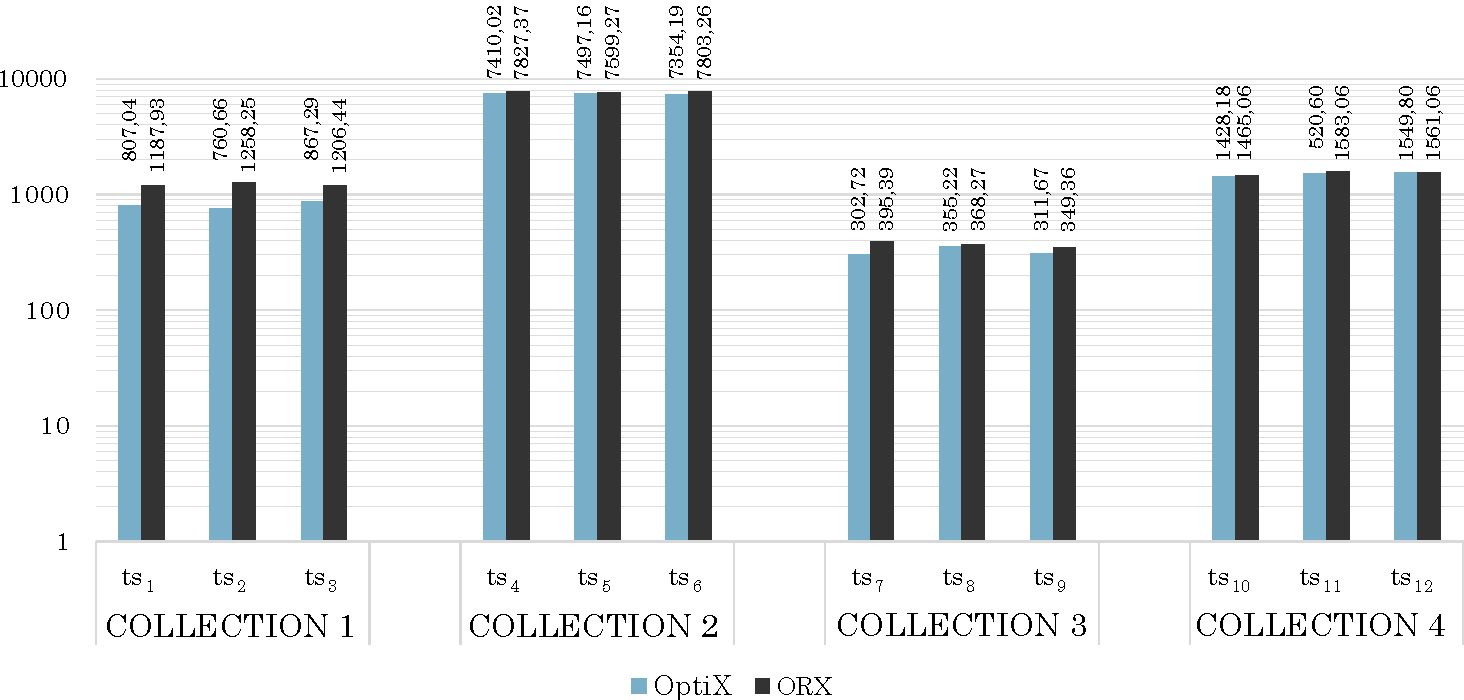
\includegraphics[scale=0.82]{figures/test_results/all.pdf}
        \caption{Complete Results from Experimental Evaluation}
        \label{fig.expres}
    \end{figure}
\end{landscape}

The complete results from the experimental evaluation are visualized in Figure \ref{fig.expres}. Because of major variations in numbers, a logarithmic scale is used in the graph. The results from each collection will subsequently be discussed individually.

\begin{figure}[t]
    \centering
    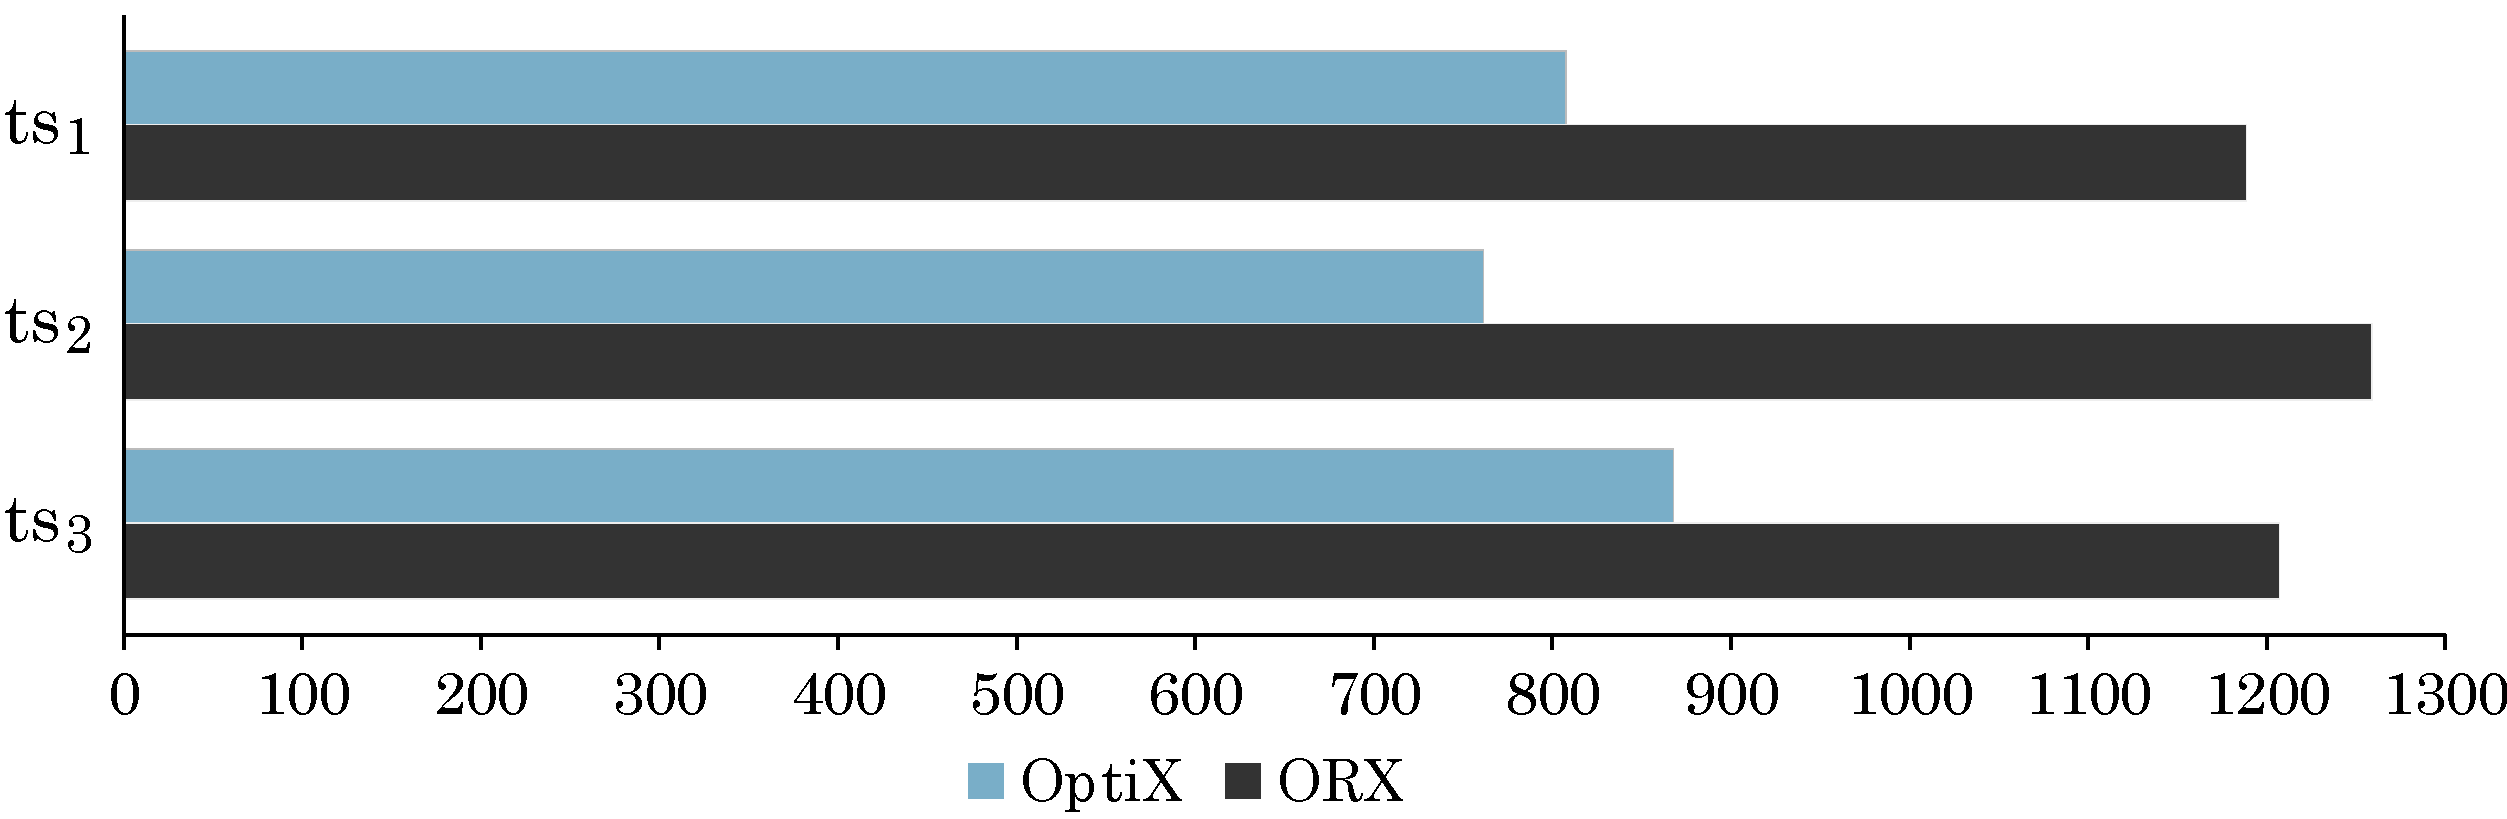
\includegraphics[width=\textwidth]{figures/test_results/1.pdf}
    \caption{Results from Test Data Collection 1 in Experimental Evaluation}
    \label{1st_test_set}
\end{figure}

The first collection of test sets consisted of $ts_1$, $ts_2$ and $ts_3$, with 1000 tests and 100 test machines. This collection was designed to test the mechanisms in situations with a large number of both tests and machines, and an abundance of possible solutions.

As we can see from Figure \ref{1st_test_set}, OptiX provided excellent results compared to ORX for these test sets. Not only were all of the execution times provided by OptiX between 305 and 472 seconds faster than ORX; it also provided better searching times. $ts_1$ was the test set with the most possible solutions, as all tests could be executed on all machines, and thus the only test set with which OptiX timed out after 30 seconds. Although the searching process of ORX timed out after 30 seconds, the whole process took just over 34 seconds in all of these cases, which can likely be explained by the post-processing time being extended as a consequence of large numbers of tests and machines. This was the collection in which the results provided by OptiX was the most prominent.

\begin{figure}[t]
    \centering
    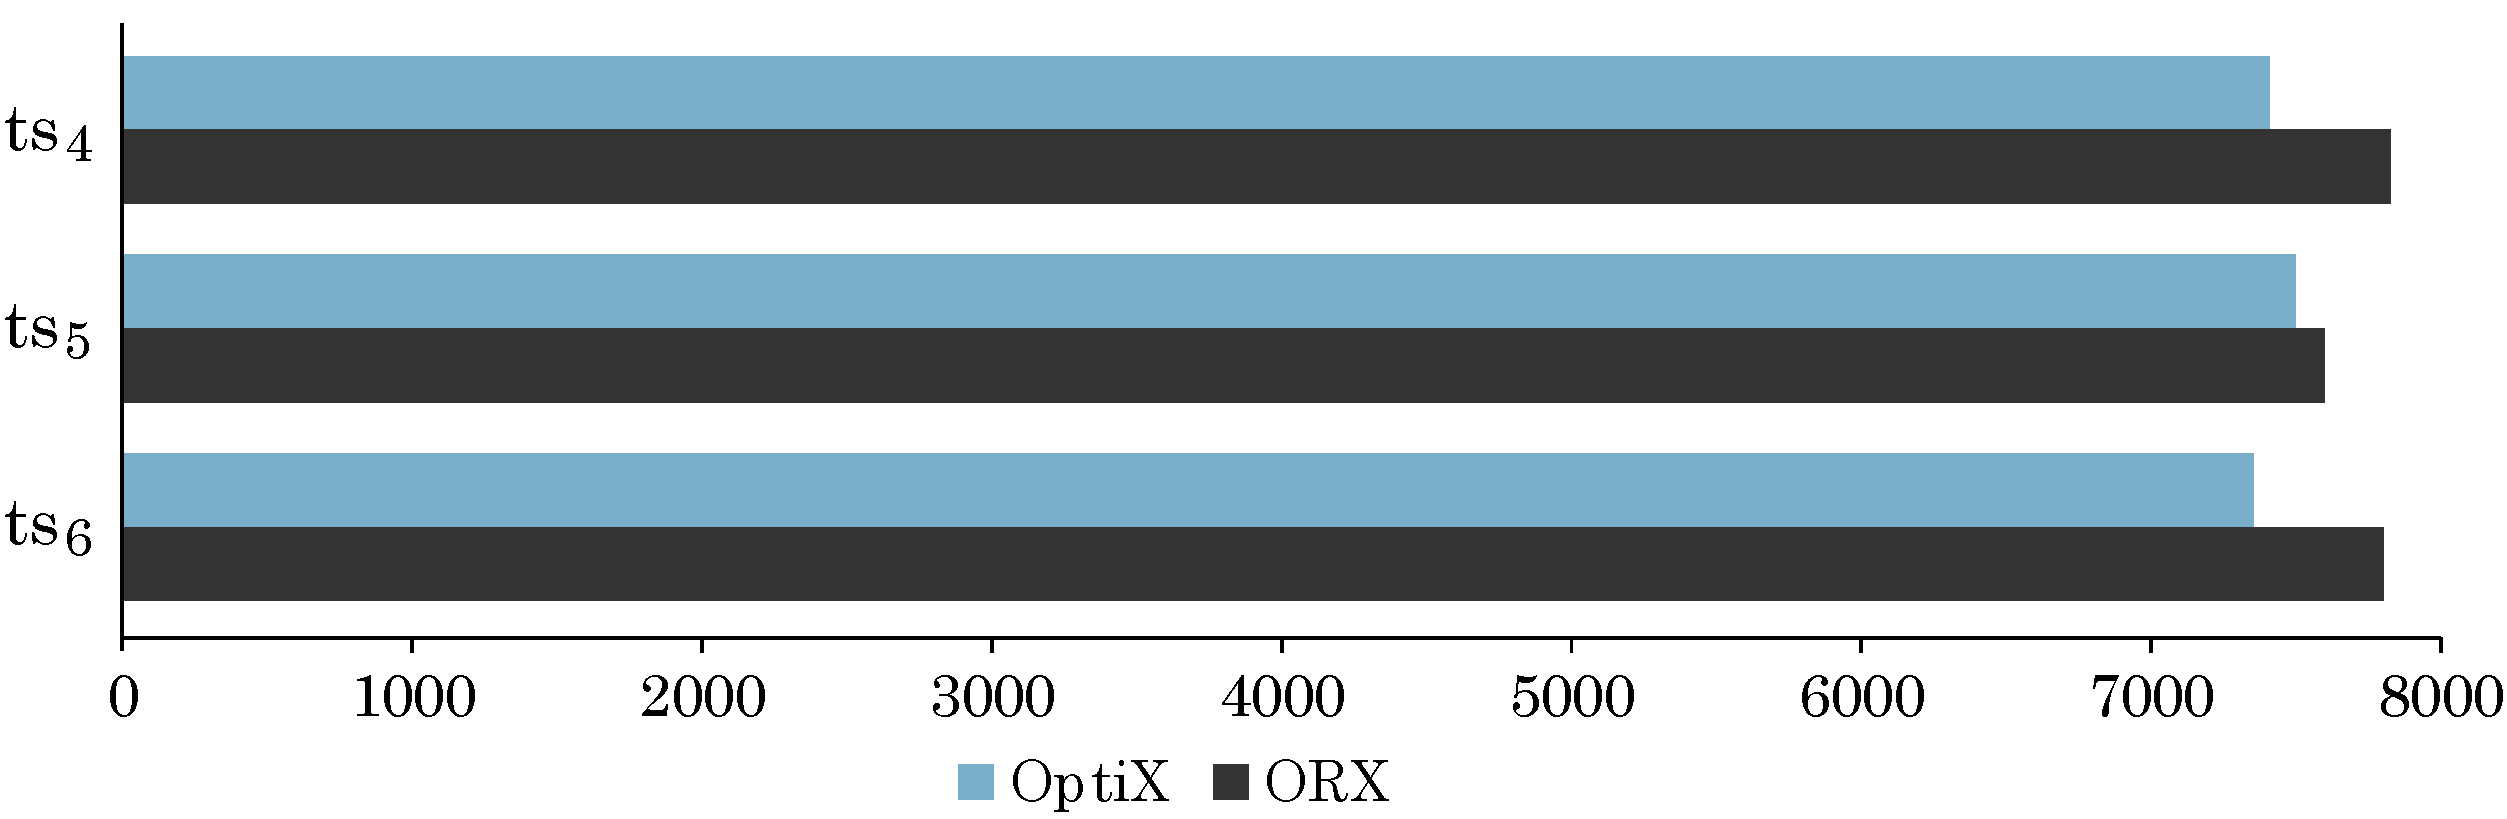
\includegraphics[width=\textwidth]{figures/test_results/2.pdf}
    \caption{Results from Test Data Collection 2 in Experimental Evaluation}
    \label{2nd_test_set}
\end{figure}

The second collection of test sets consisted of $ts_4$, $ts_5$ and $ts_6$, with 1000 tests and 10 test machines, and was designed to test the mechanisms in situations with a large number of tests and a small number of machines.

Figure \ref{2nd_test_set} shows that even though OptiX provided better total time than ORX on all test sets, the difference between the two mechanisms is less prominent in this collection than in the previous one. The largest difference in total time is 449.07 seconds for $ts_6$, and the smallest 102.11 seconds for $ts_5$, which are both small numbers considering that the total duration is more than two hours for both mechanisms on each test set. The  is likely linked to the much smaller number of possible solutions in the test sets in this collection compared to the first one. Nevertheless, OptiX undeniably outperformed ORX in searching time, where OptiX used less than a second on each test set and ORX timed out after 30 seconds, as well as in the execution time, and thus the total time on all test sets in this collection.

\begin{figure}[b]
    \centering
    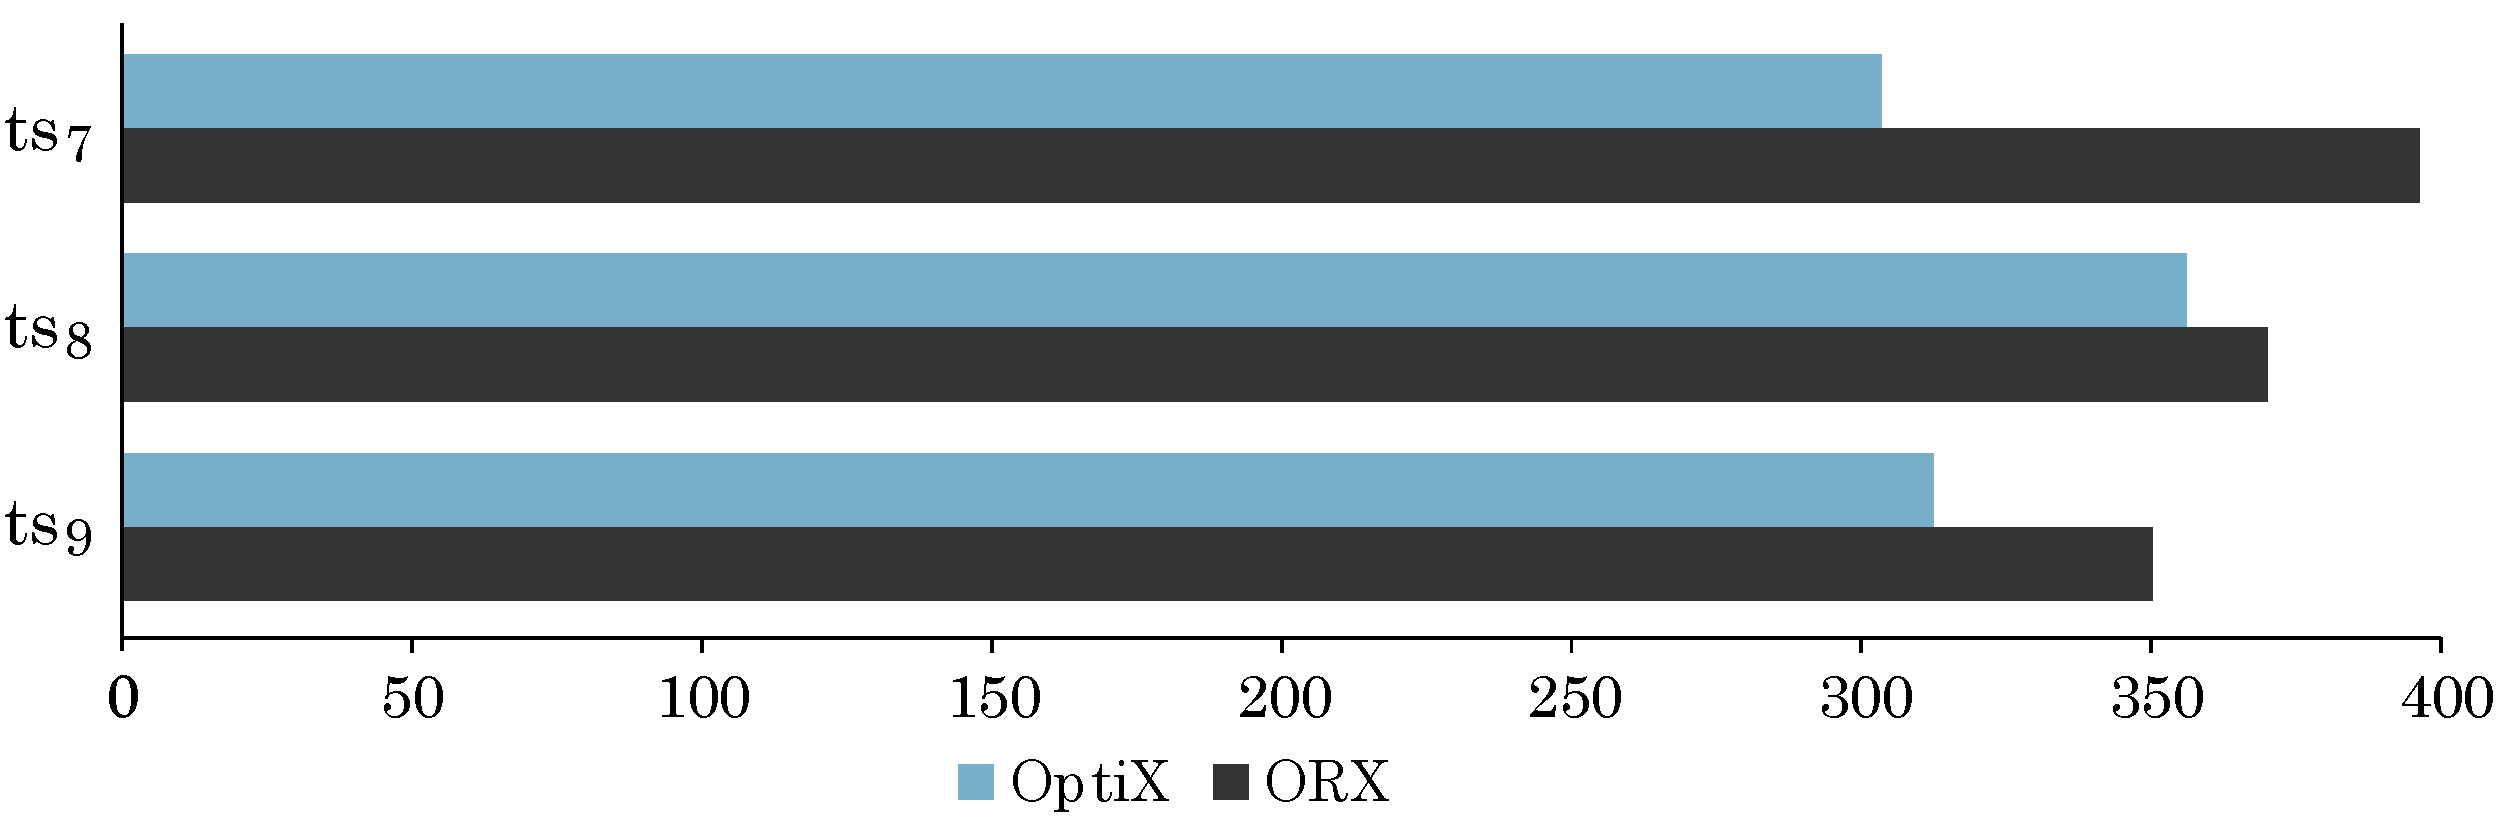
\includegraphics[width=\textwidth]{figures/test_results/3.pdf}
    \caption{Results from Test Data Collection 3 in Experimental Evaluation}
    \label{3rd_test_set}
\end{figure}

The third collection of test sets consisted of $ts_7$, $ts_8$ and $ts_9$, with 200 tests and 50 test machines, and was designed to test the mechanisms in situations with more realistically number of tests, and a fair number of machines.

Figure \ref{3rd_test_set} shows that OptiX once again provided better total results for all of the test sets in the collection. OptiX finished searching after 1.72, 0.22 and 0.67 seconds respectively for the three test sets, while ORX again was timed out after 30 seconds.

$ts_7$, which was the test set with the largest number of possible solutions, was also the one where the difference between the two mechanisms were the most distinct as the total difference was 92.67 seconds. The two remaining differences were not as conspicuous. An interesting trait that was discovered was that ORX provided a 17 second shorter execution time for $ts_8$ than OptiX accomplished. However, by using 30 seconds to find this solution, OptiX still provided a better total time. This demonstrates that it is not enough to find an allocation in which the execution time is minimized; it is also important to minimize the time taken to find the solution. 

\begin{figure}[t]
    \centering
    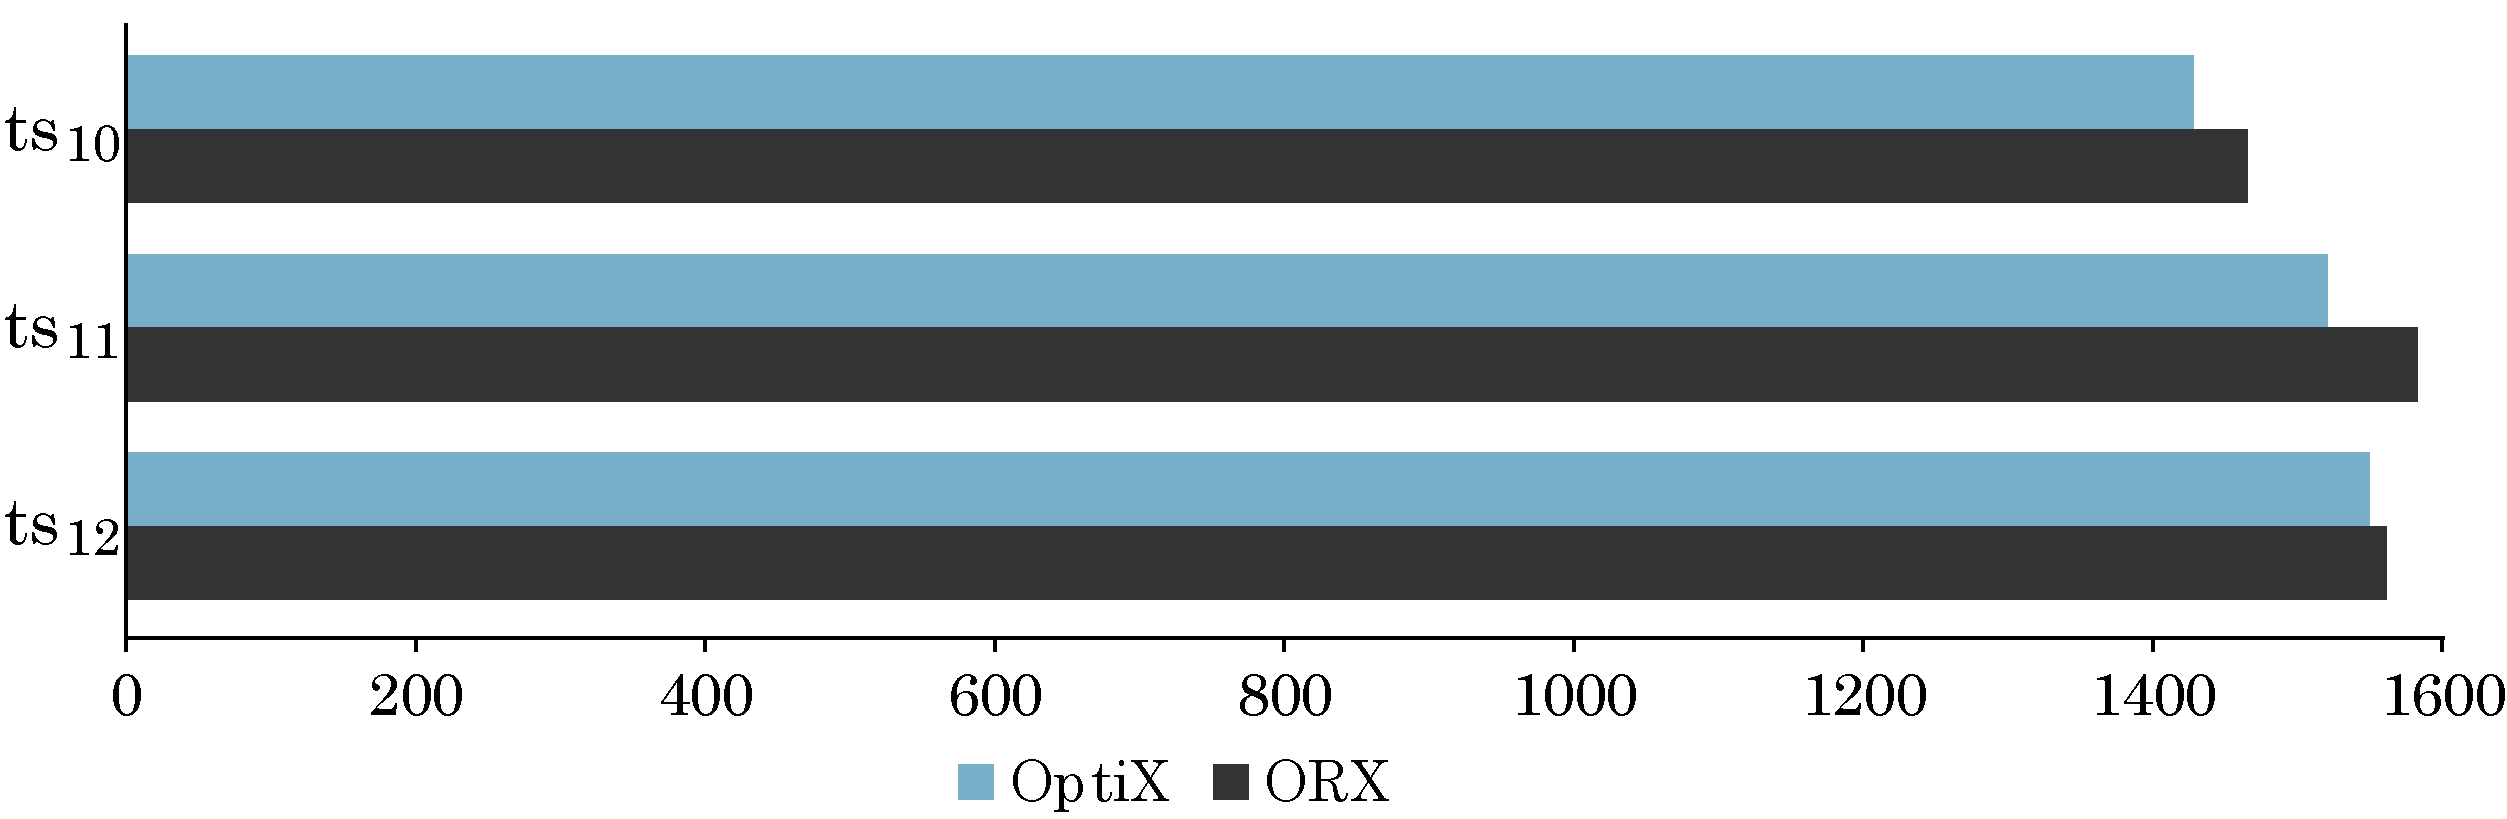
\includegraphics[width=\textwidth]{figures/test_results/4.pdf}
    \caption{Results from Test Data Collection 4 in Experimental Evaluation}
    \label{4th_test_set}
\end{figure}

The fourth and last collection of test sets consisted of $ts_{10}$, $ts_{11}$ and $ts_{12}$, with 200 tests and 10 test machines, and was designed to test the mechanisms in situations with realistic numbers of both tests and machines in terms of the context the mechanism will be used in at Altibox.

Again, OptiX produced better results for all of the test sets, which can be seen in Figure \ref{4th_test_set}. As with collection 3, the differences in results were not as outstanding for this collection as for the two first ones. This is likely due to a much more limited amount of possible solutions to the problem, as the number of test machines was small and the number of tests moderate.

The largest difference in execution time was a mere 33 seconds for $ts_{11}$. Again, ORX produced a better solution of execution time for $ts_{12}$, but since OptiX used less than a second to find its solution for this and the remaining test sets, and ORX again was timed out after 30 seconds for the whole collection, OptiX provided the overall best result of 1549.80 seconds, which was 11.26 seconds less than the total time found by ORX for this problem.

%\begin{center}* * *\end{center}
\begin{center}------------------------------\end{center}

\noindent OptiX provided better results than ORX on all of the test sets in the collection. The searching time was generally exceptional, aside from for $ts_1$, where the searching was timed out after 30 seconds, and $ts_2$, where the searching time was more than 8 seconds. Compared to the searching times of ORX, OptiX did a better job on every test set.

It is a clear trend that ORX requires a lot of time to find good results, and that the quality of the final results most of the time is poor compared those of OptiX. Both mechanisms were timed out upon solving the problem with the largest amount of combinatorial solutions, but the total time of ORX' result was nevertheless 147\% of that of OptiX'.

However, ORX found better execution times for $ts_8$ and $ts_12$, which means that even though OptiX provided better overall results, the mechanism still has potential for improvement. Although OptiX performed better that the benchmark values for all test sets, the difference between the results provided by the two mechanisms was generally not tremendous. This was especially the case for collection 4, which is the most realistic scenario covered by the experimental evaluation.

OR-tools is an excellent library for solving CP and combinatorial problems, but OptiX provided better results in this specific problem. A contributing factor to can be explained by OptiX being designed and implemented specifically to solve this type of problem efficiently, whereas OR-tools was designed to provide feasible solutions to a much broader range of problems. It is therefore not guaranteed to make the best decisions at any point of the process, so the time taken to identify good solutions is inclined to take more time. This is likely the reason why ORX did not stop before the timeout of 30 seconds on any of the test sets, whereas OptiX used less than a second on most of them.

\subsection{Threats to Validity}

Judging from the results obtained in the previous section, it is clear that OptiX is performs superior compared to ORX in the experiments. It is therefore important to establish some possible contributing factors that may threaten the validity of the results.

As explained in the previous section, the test data was randomly generated. This means that there might have been some degree of chance involved, and that if the test sets were generated again, other results may be obtained. Additionally, there might have been some interesting situations in which to test the performance of the allocation mechanisms, that are not covered in the experimental evaluation. Even though the author tried their best to come up with realistic and representative scenarios to cover the allocation mechanism in full measure, there might have been some relevant scenarios that were not tested. Also, there might be some scenarios that would provide value despite being deemed pointless to test by the author.

The results may also depend on the performance of the machine that the experiments were conducted on. Had the experiments been conducted on a newer and faster machine with more available resources or a different operating system, the results would likely come out slightly different. ORX would perhaps be able to reach better solutions before being timed out, and could thus possibly be a stronger competitor, whereas the results obtained by OptiX would not likely be affected as much, as most of the problems were solved in less than a second.

Another contributing factor may be the author's knowledge of and experience with OR-tools being far from optimal. With limited documentation and general online and literary coverage, exploring every corner of the library just could not be done with a narrow time-frame and other tasks that had to be prioritized. Although the author did invest a fair amount of time and energy in getting acquainted with the tools and tried their best to implement ORX to be as strong of a competitor to OptiX as possible, it may be a very real possibility that there are ways to implement it that would provide greater efficiency. Another possibility is that there are other optimization libraries that could potentially accomplish better results in this optimization problem than OR-tools.

\subsection{Discussion}
\improvement[inline]{TODO}
\comment{Selenium and Selenium Grid.

Noe om objektivet at prosjektet.

It is not necessary to be a highly skilled programmer to write Selenium test scripts, although some technical knowledge is required.


Egner seg spesielt godt til å kjøre store testsett og optimalisere kjøretiden

}












\subsection{Return on Investment}

Altibox has great interest in how incorporating \toolname \space to their testing process can affect their company from a business perspective. This section aims to enlighten some of these aspects.

All of the frameworks used in the development of \toolname \space are open-source. It has therefore not been necessary to pay for any licenses. \toolname \space itself is also handed to Altibox with no charges, so the associated investment solely consists of time and resources.

A priority during the design phase has been to create a user-friendly, intuitive and consistent interface. Building the website on the Django framework has rendered this an easy task. Getting to know the interface and learning to use it is thus not expected to be require excessive amounts of time and effort. Also, a brief user manual is included both on the website and in the appendix of this thesis.

As with test automation in general, writing test scripts for \toolname \space requires some technical knowledge. Being acquainted with the Python programming language and the Selenium library is a necessity. Writing these scripts will also take time, and additional time associated with maintaining said scripts should be expected. Furthermore, at least one computer, preferably more, should be available solely to be used for \toolname.

The success of applying \toolname \space partially depends on how the product is used. As explained in Chapter \ref{chapter.background}, caution should be used upon determining the automation coverage and which exact test that should be automated. The media content in TV Overalt is dynamic, as new movies and TV shows are released and made available, while old content is removed after a while. Thus, content-based tests are not likely to be durable, and will presumably require regular maintenance. Attempting to automate everything is also an approach that is almost guaranteed to fail \cite{ksljdf}.

But there are a lot of benefits to \toolname \space too, if used correctly. One of these benefits is significantly extended test coverage. Currently, TV Overalt is available in Chrome, Edge, Firefox, Internet Explorer and Safari. During an acceptance test, the test team often has limited amount of time, which means that they will not be able to perform all of the tests in all browsers, and have to select which browsers should be tested. This will most likely no longer be a problem after incorporating \toolname, as each test script can be executed in all of these browsers. Once the test scripts are written and in working order, they can be executed rapidly, precisely and repeatedly with no additional expenses and virtually no time used by human resources, and in \improvement{Except Safari?} all of the aforementioned browsers with only a few keystrokes. The remaining time can thus be used for manually conducting the tests unsuited for automation. This way, it will now be possible to cover all of the supported browsers even with a limited time frame, and thus be able to test the test object more thoroughly and detect more defects.

Detecting more defects will likely result in improved product quality, and by extension additional time to test the product to an even greater extent. Other effects of this could be fewer customer inquiries and higher customer satisfactory, which could lead to increased customer confidence in the product as well as in the company.

Another strength to \toolname \space is that even though developing test scripts is a task that requires technical staff, once the scripts are written and uploaded, no technical background is needed to execute the tests, which would be the case without the user interface of \toolname.

As explained in the previous section, writing Selenium tests generally does not require advanced programming skills and is not immensely time-consuming. The code involved is fairly simple, as it is mostly compromised of locating web elements based on the class or id names, or similar, of the elements in the HTML code, and clicking buttons or filling out text fields. The time used for test script coding and maintenance will likely take approximately the same amount of time as a few manual executions of the same test, and thus provide great value in the long term.

As opposed to some other cloud testing services which execute tests on remote machines in distant locations, \toolname \space can execute tests on un-deployed versions of the test object, that are only available on the network that the \toolname \space server is connected to. In practice, this means that the tests uploaded to \toolname \space can be executed on the test object before it is deployed, and thus be able to identify defects earlier.

\toolname \space provides a JIRA integration that will enable the testers to save a lot of time on reporting failed test executions to the issue tracking system, which will be of great value. Locating issues linked to a specific test can also be done without having to open the JIRA website and search for issues with specific attribute values that comply with the specific test.










\comment{- What is needed in order for the product to be used (Learning to set up and use the tool, dedicated machines, learning to write automated tests and learning to use optiruns template for automated tests, learning python if they don't know it already)
- Was it worth it (for Altibox)?
- How optirun competes with alternative tools
- Compare to current test process?


This chapter will include:\\
- Research questions\\
- Thorough performance comparison of optx and orx - use graphs!\\
- Evaluation of allocation mechanism\\
- Discussion of complete system\\
- Discussion of how \toolname \space can affect Altibox' overall testing process of TV Overalt (time saved or more time used to write tests? Human mistakes avoided if tests are written well, etc.). Compare to how the test process has previously been.


The existing test process will be discussed in Chapter \ref(chapter.discussion).
Test automation has previously been completely omitted, and Altibox was avid to include this in the testing of their software products.
}


\section{Further Work \& Conclusion}\label{chapters.conclusion}
\thispagestyle{plain}

\subsection{Further Work}
\improvement[inline]{TODO}
\comment{
    Further work:
    Integrate CI environment!
    Include app testing (appium)
    Include STB testing (WitBe)
    Include web streaming testing (WitBe)
    Create mobile notification app (if Android is created as part of the thesis, future work can include iOS version. Otherwise maybe a cross-platform app?)
}

\subsection{Conclusion}
\improvement[inline]{TODO}

    
\renewcommand\thesection{\Alph{section}}
\setcounter{section}{0}

\section{Setup}
\thispagestyle{plain}
\improvement[inline]{TODO}

\comment{
\todo[inline]{Complete setup instructions}

\subsection{Virtual Machine Setup}

\subsection{Server Setup}
\subsubsection{Installing required packages}

\subsection{Test Machine Setup}
}
%\section{Test Data}
\thispagestyle{plain}
\improvement[inline]{TODO}
\comment{One page for each test set; one table and one or two graphs? plus maybe some other facts? Average test duration? Best case scenario total duration? Number of machines? Number of tests? Number of machines each test is executable on? Opti-X result and OR-X result?}
\section{Automated Test Template}
\thispagestyle{plain}
\comment{One page for each test set; one table and one or two graphs? plus maybe some other facts? Average test duration? Best case scenario total duration? Number of machines? Number of tests? Number of machines each test is executable on? Opti-X result and OR-X result?}

This template for automated test scripts should be strictly conformed to:
    
\begin{lstlisting}[caption=Template for Automated Test Scripts, label={listing.test_template}]
import json
import sys
import unittest
from selenium import webdriver

class NameOfTest(unittest.TestCase):
    @classmethod
    def setUpClass(cls):
        data = json.loads(sys.argv[1])

        cls.driver = webdriver.Remote(
            command_executor=data['command_executor'],
            desired_capabilities=data['desired_capabilities']
        )

    def name_of_test(self):
        """ Write the test script here """

    @classmethod
    def tearDownClass(cls):
        if cls.driver is not None:
            cls.driver.quit()

if __name__ == "__main__":
    unittest.main(argv=['TestCase'])
\end{lstlisting}


% Inserting list of figures and list of tables. Remove \newpage between lists if they can fit in one page (compile to check)

    %\comment{
        \thispagestyle{plain}
        %\onehalfspacing
        \renewcommand{\listfigurename}{Figures}
        %\listoffigures
        \newpage
    %}
    
    \comment{
        \thispagestyle{plain}
        \listoftables
        \newpage
    }
    
    %\comment{
        \thispagestyle{plain}
        \renewcommand{\lstlistlistingname}{\lstlistingname s}
        \lstlistoflistings
        \newpage
    %}
    
    % Inserting references, again with custom line spacing (setstrech) to avoid odd page breaks or fit to whole pages
    \small
    \setstretch{.8}
    %\bibliographystyle{unsrtnat}		%Inserting bibliography
    %\bibliographystyle{IEEEtran}
    \clearpage
    \thispagestyle{plain}
    \bibliographystyle{plain}
    \bibliography{doc_files/references}
    \newpage



\end{document}						%End of document

